\documentclass[11pt,a4paper,oneside]{report}
\usepackage{fontspec}
\usepackage{geometry}
% 13cm measure, about 72 characters at 11pt. The outer margin is deliberately generous:
% it is a named column that the wide figures are set into, not slack.
\geometry{
  a4paper,
  top=2.7cm, bottom=2.9cm, left=3.2cm, right=2.8cm,
  marginparwidth=2.0cm, marginparsep=0.4cm,
  headsep=0.7cm, footskip=1.2cm
}
\usepackage{booktabs}
\usepackage{tabularx}
\newcolumntype{L}{>{\raggedright\arraybackslash\hspace{0pt}}X}
\newcolumntype{R}{>{\raggedleft\arraybackslash\hspace{0pt}}X}
\usepackage{graphicx}
\usepackage{microtype}
\usepackage[table]{xcolor}
\usepackage{titlesec}
\usepackage{fancyhdr}
\usepackage{parskip}
\usepackage{caption}
\usepackage{float}
\usepackage{chngcntr}
\usepackage{fancyvrb}
\usepackage{enumitem}
% Figures and tables are numbered straight through rather than per chapter, so the numbers
% match the captions in the markdown sources and any reference to them in the body text.
\counterwithout{figure}{chapter}
\counterwithout{table}{chapter}

\definecolor{srhorange}{HTML}{E64415}
\definecolor{ink}{HTML}{1A1A1A}
\definecolor{slate}{HTML}{555555}
\definecolor{hair}{HTML}{C9C6C0}

\linespread{1.06}
\setlength{\parskip}{0.55em}
\widowpenalty=10000
\clubpenalty=10000
\setlist{noitemsep, topsep=4pt, parsep=2pt, leftmargin=1.5em}

% Interactive navigation, which is the point of this build: TOC entries, figure and
% section references, and the reader's sidebar all become links. Internal links are ink
% rather than orange: they are navigation, and colouring every one of them turns the
% contents page into a field of accent colour. External DOIs stay orange, because there
% the colour is telling the reader the link leaves the document.
\usepackage[
  colorlinks=true, linkcolor=ink, citecolor=ink, urlcolor=srhorange,
  bookmarks=true, bookmarksopen=true, bookmarksnumbered=true,
  pdftitle={Probabilistic Day-Ahead Solar Forecasting and Risk-Aware Battery Dispatch under Concept Drift}, pdfauthor={Devendra Singh Dhakad},
  pdfsubject={Case Study 1, SRH University of Applied Sciences Heidelberg}
]{hyperref}

% Contents entries without dotted leaders. \@dotsep is a length in mu; setting it absurdly
% large suppresses the dots without pulling in another package.
\makeatletter
\renewcommand{\@dotsep}{10000}
\makeatother

\captionsetup{
  font=small, labelfont=bf, labelsep=period,
  singlelinecheck=false, justification=raggedright, skip=8pt
}
\captionsetup[table]{position=top, skip=6pt}

\titleformat{\chapter}[display]
  {\normalfont\huge\bfseries\color{ink}}
  {\color{srhorange}\normalsize\bfseries\MakeUppercase{\chaptertitlename\ \thechapter}}
  {10pt}{\Huge}[\vspace{8pt}{\color{hair}\titlerule[0.6pt]}]
\titlespacing*{\chapter}{0pt}{34pt}{30pt}
\titleformat{\section}{\normalfont\large\bfseries\color{ink}}{\thesection}{0.6em}{}
\titlespacing*{\section}{0pt}{20pt}{6pt}
\titleformat{\subsection}{\normalfont\normalsize\bfseries\color{ink}}{\thesubsection}{0.6em}{}
\titlespacing*{\subsection}{0pt}{14pt}{4pt}

\pagestyle{fancy}
\fancyhf{}
\renewcommand{\headrulewidth}{0.4pt}
\renewcommand{\headrule}{{\color{hair}\hrule height \headrulewidth width\headwidth}}
\fancyhead[L]{\small\color{slate}\nouppercase{\leftmark}}
\fancyhead[R]{\small\color{slate}\thepage}
\renewcommand{\chaptermark}[1]{\markboth{\thechapter\quad #1}{}}
\fancypagestyle{plain}{%
  \fancyhf{}%
  \renewcommand{\headrulewidth}{0pt}%
  \fancyfoot[C]{\small\color{slate}\thepage}%
}

% Code and the architecture block: smaller, with a hairline in the margin so it reads as
% an inset. No commandchars, because the block contains literal backslashes and arrows.
\DefineVerbatimEnvironment{codeblock}{Verbatim}{%
  fontsize=\footnotesize, frame=leftline, framerule=1.2pt,
  rulecolor=\color{hair}, framesep=9pt, xleftmargin=12pt
}

% The pre-registered prediction in 5.1 is quoted rather than paraphrased, and it is the
% one block quote that carries an argument, so quotes get a hairline and an indent rather
% than the class default.
\newenvironment{pullquote}
  {\begin{list}{}{\setlength{\leftmargin}{1.4em}\setlength{\rightmargin}{0pt}}\item[]%
   \itshape\color{ink}}
  {\end{list}}

\setlength{\emergencystretch}{3em}
\sloppy

\begin{document}

\begin{titlepage}
\thispagestyle{empty}
\centering

\includegraphics[width=4.2cm]{assets/srh_logo.jpg}
\vspace{1.6cm}

{\color{srhorange}\rule{\linewidth}{1.2pt}}
\vspace{1.0cm}

{\LARGE\bfseries Probabilistic Day-Ahead Solar Forecasting and Risk-Aware Battery Dispatch under Concept Drift\par}
\vspace{1.0cm}
{\color{srhorange}\rule{\linewidth}{1.2pt}}

\vspace{1.6cm}
{\large Case Study 1\par}
\vspace{0.4cm}
{\color{slate}\large September 2026\par}
\vspace{2.4cm}

\begin{tabular}{@{}rl@{}}
\textbf{Author}         & Devendra Singh Dhakad \\[4pt]
\textbf{Matriculation}  & 100004684 \\[4pt]
\textbf{Programme}      & M.Sc. Data Science and Artificial Intelligence \\[4pt]
\textbf{Supervisor}     & Prof. Dr. Mehrdad Jalali \\[4pt]
\textbf{University}     & SRH University of Applied Sciences Heidelberg \\
\end{tabular}

\vfill
\end{titlepage}

\pdfbookmark[0]{Contents}{toc}
\tableofcontents
\clearpage
\pdfbookmark[0]{List of Figures}{lof}
\listoffigures
\clearpage


\chapter{Introduction}

\section{Motivation}

Photovoltaic capacity is being added to European grids faster than the tools for scheduling around it are maturing. Germany, the setting for this study, roughly doubled its installed PV fleet over the five years covered by the dataset used here. Every megawatt of that fleet has to be scheduled a day in advance, because the European day-ahead market closes at noon for delivery across the whole of the following day. An operator who commits to a schedule and then fails to meet it does not receive a lower score; the operator pays an imbalance penalty, and the penalty for being short is typically several times the penalty for being long.

That asymmetry is the reason this report is organised the way it is. A forecast is an input to a decision, and the decision is settled in money rather than in mean absolute error. Once the costs of over- and under-delivery differ, the cost-minimising commitment is no longer the expected value of tomorrow's generation. It is a quantile of the predictive distribution, and which quantile depends on the ratio of the two penalties. A point forecast, however accurate, cannot express that quantity at all: it reports one number where the decision needs a shape.

\section{The gap this work addresses}

Two literatures exist and rarely meet. The forecasting literature produces increasingly sophisticated probabilistic models and evaluates them with proper scoring rules. The power-systems literature produces stochastic optimisation formulations and evaluates them under assumed distributions. Papers that run an actual forecasting pipeline into an actual dispatch problem and report what the forecast was worth in currency are comparatively rare, and papers that ask whether the ranking by scoring rule survives the translation into the ranking by cost are rarer still.

A second gap is practical. Most published day-ahead PV forecasters consume numerical weather prediction (NWP) input. That is the right choice when the input is available, but it is not available to a small operator who cannot buy a commercial forecast feed, and it obscures how much of the achievable skill comes from the weather model rather than from the machine learning. This study therefore imposes an NWP-free constraint deliberately, replacing the weather input with what is free: the analytic astronomy of the sun's position and a clear-sky irradiance model.

A third gap concerns validity rather than accuracy. Quantile regression produces intervals that are sharp but carry no coverage guarantee, and the guarantee that conformal prediction supplies rests on exchangeability, which a strongly seasonal series violates by construction. Whether the classical split-conformal procedure survives a twelve-month test period, and what to do when it does not, is an empirical question this study is in a position to answer.

\section{Research questions}

\textbf{RQ1.} How much day-ahead forecasting skill is available without any NWP input, and does conformal calibration deliver valid coverage under the seasonal non-stationarity of a solar series?

\textbf{RQ2.} Does a better forecast score buy a better decision? Specifically, what is the euro value of committing against a full predictive distribution rather than a point forecast, and how does the ranking of models by CRPS compare with their ranking by dispatch cost?

\textbf{RQ3.} At an equal retraining budget, does retraining triggered by a drift detector outperform retraining on a fixed calendar?

\textbf{RQ4.} What information does the fitted model actually depend on, and is the attribution reported by SHAP the same thing as necessity?

\textbf{RQ5.} A newly commissioned site has days of history rather than years, but must still submit a schedule tomorrow. How much local history is needed before training on it beats borrowing a model trained on a different country, and does combining the two do better than either?

\section{Contributions}

This report contributes an end-to-end, reproducible pipeline that runs a leakage-audited day-ahead forecasting stage into a two-stage stochastic dispatch problem and reports the outcome as regret against a perfect-foresight oracle. Within that pipeline it contributes: a physics-informed, NWP-free feature construction whose leakage-safety is verified by an adversarial test rather than by inspection; a comparison of raw and conformalised predictive intervals across six model families; a quantification of the relationship between forecast score and decision value across twenty model variants; a budget-matched comparison of retraining policies; and a side-by-side comparison of SHAP attribution against leave-one-family-out ablation.

On the small-data question it contributes a four-way comparison -- local-only, zero-shot transfer, source-plus-local-correction, and pooled training -- run across three target countries spanning nine degrees of latitude, with the crossover point reported as the quantity of operational interest.

It also contributes a documented account of five defects found during development, each of which produced a plausible but wrong result, together with the methods that exposed them. Two of the five were caught only because naive baselines were carried through to the final table.

\section{Structure of this report}

Chapter 2 reviews the state of the art across the four areas the study touches. Chapter 3 sets out the methodology: the day-ahead protocol, the data, the leakage-safe feature construction, the models, the evaluation design and the dispatch formulation. Chapter 4 describes the implementation. Chapter 5 reports results against each research question. Chapter 6 discusses what the results mean, including a hypothesis the data refuted. Chapter 7 states the limitations, and Chapter 8 concludes.


\chapter{State of the Art}

\section{Photovoltaic power forecasting}

Antonanzas et al. (2016) survey the field and separate approaches by the input they consume: persistence and statistical time-series methods that use only the generation history, machine-learning methods that add exogenous variables, and physical methods driven by NWP. Their review makes clear that the choice of input dominates the choice of model class at day-ahead horizons, because beyond a few hours the autocorrelation of cloud cover has decayed and the remaining information is meteorological.

That observation sets the ceiling for the present work. Without NWP, a day-ahead PV forecaster knows the deterministic diurnal and seasonal envelope exactly, and knows the recent state of the atmosphere, but has no direct information about tomorrow's clouds. The realistic expectation is therefore a modest improvement on seasonal persistence rather than a large one, and any study reporting a large improvement without NWP should be examined for leakage before it is believed.

The deterministic envelope itself is not a modelling problem but an astronomical one. Reda and Andreas (2004) give the standard solar position algorithm; Haurwitz (1945) and Ineichen and Perez (2002) give clear-sky irradiance models of very different vintage and complexity, and Kasten and Young (1989) give the relative air mass on which the latter depends. Normalising observed output by a clear-sky expectation to obtain a clear-sky index is long-standing practice in solar resource assessment, and it is attractive here because it removes the deterministic cycle before learning begins.

\section{Probabilistic forecasting and its scoring}

Gneiting and Katzfuss (2014) survey probabilistic forecasting and articulate the principle the evaluation in this report follows: maximise sharpness subject to calibration. Gneiting and Raftery (2007) formalise the scoring rules that make the principle operational, and establish which rules are proper, meaning that the forecaster's expected score is optimised by reporting the true predictive distribution. The continuous ranked probability score (CRPS) is the proper rule used here, evaluated through its quantile decomposition so that it can be computed from a quantile grid.

Two supporting rules matter. Koenker and Bassett (1978) introduced the quantile loss whose minimiser is the corresponding quantile, which is both the training objective of the quantile models in this study and the per-level component of CRPS. Winkler (1972) introduced the interval score, which penalises width and miss distance together and therefore cannot be improved by widening an interval. That property is the reason this report never presents coverage without an interval score beside it.

In the energy domain specifically, van der Meer, Widén and Munkhammar (2018) review probabilistic forecasting of PV production and consumption, and Hong et al. (2016) describe the Global Energy Forecasting Competition 2014, which established probabilistic track formats and quantile-based evaluation as the norm for the field. Bremnes (2004) and Pinson (2012) are representative of the quantile-regression and parametric-distribution strands respectively in wind power, and Wang et al. (2017) apply deep convolutional architectures to deterministic and probabilistic PV forecasting.

\section{Distribution-free calibration}

Conformal prediction, developed by Vovk, Gammerman and Shafer, supplies finite-sample coverage guarantees under exchangeability alone, with no distributional assumption. Angelopoulos and Bates (2023) give an accessible modern treatment. Romano, Patterson and Candès (2019) combine the idea with quantile regression to produce conformalised quantile regression (CQR), which inherits the adaptive width of a quantile model and the coverage guarantee of conformal prediction; this is the split-conformal procedure used in Chapter 5.

The exchangeability assumption is the weak point for time series with seasonal structure, because a calibration slice drawn from one part of the year is not exchangeable with a test period drawn from another. Gibbs and Candès (2021) address exactly this by updating the miscoverage level online in response to observed misses, restoring long-run coverage under arbitrary distribution shift. Their adaptive conformal inference is used in Chapter 5 to close the gap that split conformal leaves open. Chernozhukov, Fernández-Val and Galichon (2010) supply the rearrangement result that repairs quantile crossing, a routine failure of independently fitted quantile models.

\section{Forecast value and decision-focused evaluation}

The observation that forecast quality and forecast value are distinct goes back at least to Murphy's work on forecast verification, and it has a clear expression in energy. Pinson, Chevallier and Kariniotakis (2007) show how a wind producer trading in a day-ahead market with asymmetric imbalance penalties should bid a quantile of the predictive distribution determined by the penalty ratio, rather than the expected value, and quantify the revenue gain. Morales et al. (2014) develop the stochastic-programming machinery for renewables in electricity markets more generally, including the two-stage structure with recourse that this report adopts.

The optimisation itself is standard. Rockafellar and Uryasev (2000) give the linearisation that makes conditional value-at-risk tractable as a linear program, which is what allows the risk-averse policy here to be solved with the same solver as the risk-neutral one. Huangfu and Hall (2018) describe the dual revised simplex implementation underlying HiGHS, the solver used.

\section{Concept drift and monitoring}

Gama et al. (2014) survey concept drift adaptation and provide the taxonomy of detectors used here. Bifet and Gavaldà (2007) introduce ADWIN, an adaptive-windowing detector with a Hoeffding-style bound on the difference of means between two windows; the Page-Hinkley test is the classical cumulative-deviation alternative. Both are designed for streams, and both threshold absolute deviations, a property that turns out to matter a great deal in Chapter 5.

\section{Explainability for tabular models}

Lundberg and Lee (2017) unify several attribution methods under the Shapley value and give an exact algorithm for tree ensembles, which is the method used here. The gradient-boosting implementations themselves are due to Chen and Guestrin (2016) and Ke et al. (2017). What the literature is less clear about, and what Chapter 5 examines empirically, is the relationship between attribution and necessity when features are redundant.

\section{Transfer learning and the small-data case}

Pan and Yang (2010) give the standard taxonomy of transfer learning, and Ben-David et al. (2010) the theoretical account of when transferring between domains can help: the achievable target error is bounded by the source error plus a divergence between the two domains plus the error of the best joint hypothesis. The practical reading is that transfer is worth attempting when the domains differ in ways the representation can absorb.

That condition is unusually favourable here. A PV site differs from another PV site mainly in latitude, orientation and installed capacity, and all three are handled before the learner sees anything: capacity by normalisation, latitude and orientation by recomputing the solar geometry for the target's own coordinates. What is left to transfer is the relationship between recent atmospheric state and tomorrow's output, which is far more portable than the raw series.

In the energy literature the newly-commissioned plant is the canonical instance of the problem. Luo, Zhang and Zhu (2022) combine transfer learning with a constrained LSTM for power forecasting at newly-constructed photovoltaic plants, and the same framing recurs for new wind farms. What is less commonly reported is the quantity an operator actually needs: not that transfer helps, but how many days of local history it is worth, which is what Section 5.5 measures.

\section{The gap}

The pieces above exist separately. What is scarce is a study that carries one dataset through all of them: an audited NWP-free forecaster, calibrated both classically and adaptively, evaluated by proper scoring rules and then again by the cost of the decisions it drives, with the drift and explainability questions asked on the same pipeline rather than on a different one. That is the gap this report addresses.


\chapter{Methodology}

\section{The day-ahead protocol}

The operational setting is the European day-ahead arrangement. At 12:00 UTC on day $D$ the operator must submit an hourly grid exchange schedule covering all twenty-four hours of day $D+1$. Forecast horizons therefore run from twelve hours (delivery hour 00:00) to thirty-five hours (delivery hour 23:00), and every hour of the delivery day is decided at the same moment on the basis of the same information.

\begin{figure}[H]
\centering
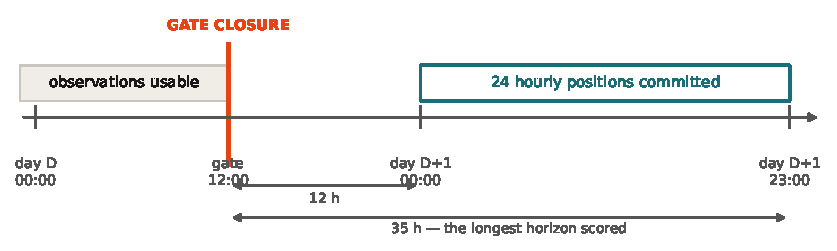
\includegraphics[width=\linewidth]{../figures/day_ahead_protocol.pdf}
\caption{The day-ahead protocol drawn to scale on a 48-hour axis. Everything to the left of the gate is usable; everything to the right is being predicted. The single most consequential property of the feature construction is that no feature may cross the orange line, and the horizon band that follows from a noon gate is 12 to 35 hours rather than the 1 to 24 that an unstated protocol would imply.}
\label{fig:protocol}
\end{figure}

Two things follow. First, the horizon band is 12 to 35 hours, not 1 to 24; reporting a day-ahead study on a 1 to 24 hour band silently assumes a gate that does not exist in this market. Second, and more dangerous, the familiar lag $y_{t-24}$ is illegal for every delivery hour after noon, because that observation is made after the schedule has already been submitted. Section 3.4 describes how this is handled and Section 4.6 how it is verified.

\section{Data}

The dataset is the Open Power System Data hourly time-series package for Germany, an openly licensed (CC-BY 4.0) compilation of ENTSO-E transparency data. It provides PV generation, wind generation, load, day-ahead price and reported installed capacity on a single hourly clock. The specific package version resolved and used here is the 2020-10-06 release of \texttt{time\_series\_60min\_singleindex}.

Quality control clips physically impossible negatives, forward-fills the irregularly reported capacity series, and interpolates gaps of at most three hours. Longer gaps are deliberately left as missing rather than filled: manufacturing a week of generation data would manufacture skill the model does not have. The analysis is then restricted to the longest contiguous span of valid target values, giving \textbf{33{,}192 hourly records over 1{,}383 complete delivery days}, from 2016-12-18 to 2020-09-30.

\begin{figure}[H]
\centering
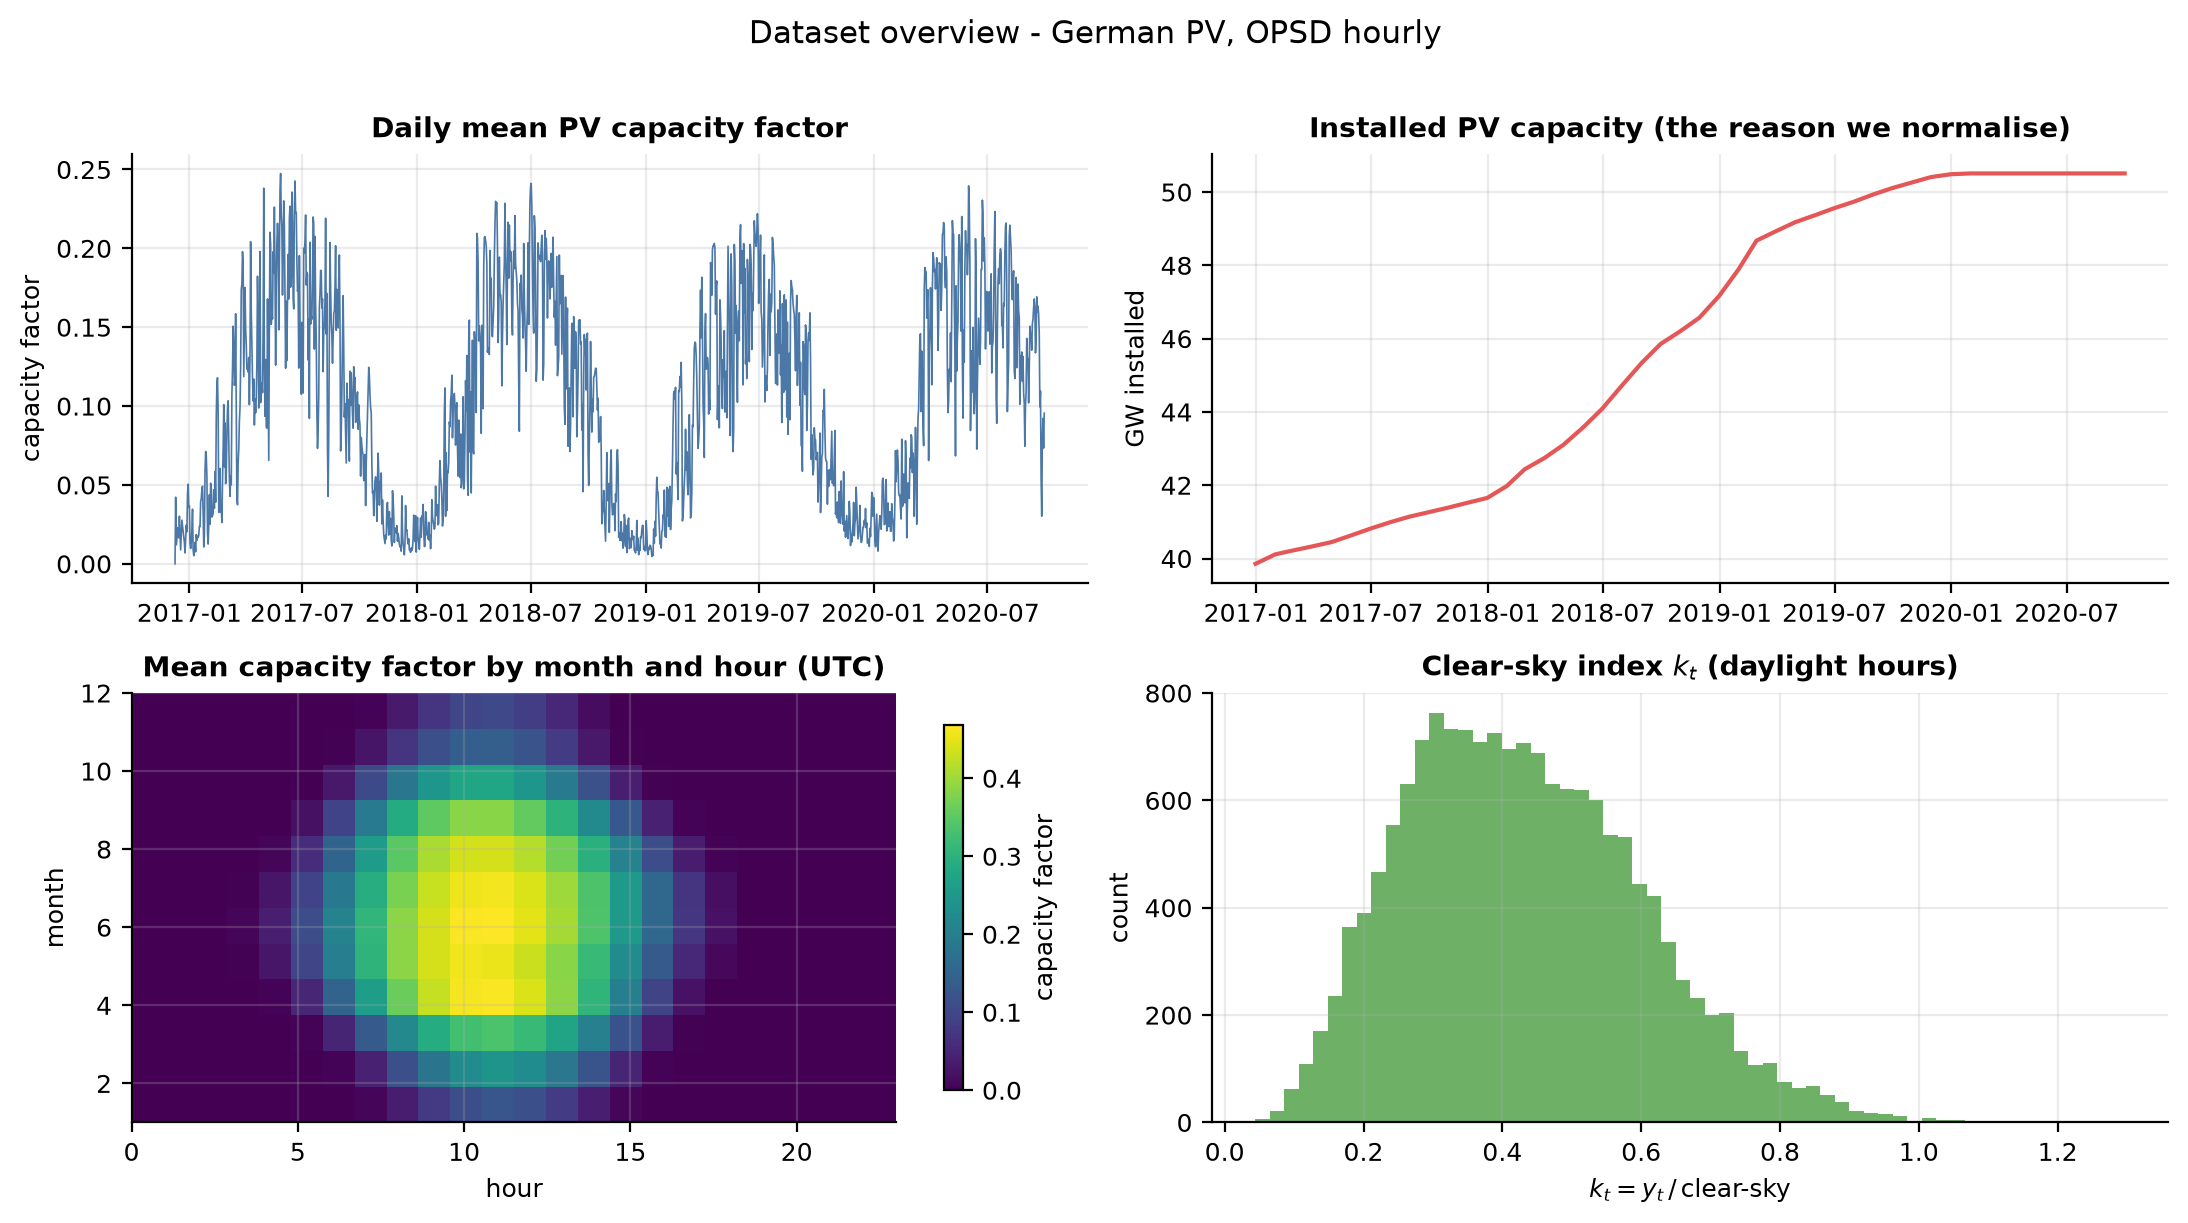
\includegraphics[width=\linewidth]{../figures/01_data_overview.png}
\caption{The dataset. Clockwise from top left: daily mean capacity factor across the sample; reported installed capacity, which grew from 39.7 to 50.5 GW and is the reason the target is normalised; mean capacity factor by month and hour, showing the deterministic envelope the physical features encode; and the distribution of the clear-sky index over daylight hours, which is the quantity the models actually have to learn.}
\label{fig:data_overview}
\end{figure}

\subsection*{Capacity normalisation, and where it is not available}

Installed German PV capacity grew by roughly 27 percent across the sample. Modelling raw megawatts would embed a deterministic upward trend in the target, which would flatter any model carrying a trend term and would contaminate the concept-drift experiment of Chapter 5 with what is in truth an accounting change rather than a change in the physical process. The target is therefore a \emph{capacity factor} in $[0,1]$, formed by dividing generation by the reported installed capacity at that timestamp.

Germany turns out to be the only zone in this package where that is possible. Checking each candidate zone's peak generation against its own reported capacity shows Switzerland at 2.94 times, Denmark at 1.81 and Great Britain at 1.37: generation above nameplate is not physically possible, so in those zones the capacity column describes a different scope from the generation column and cannot serve as a denominator. The transfer study of Section 5.5 therefore normalises every site, Germany included, by the 99.9th percentile of its own generation, which is a well-defined robust scale that puts all sites on a comparable $[0,1]$ footing. It is not a capacity factor and is not labelled as one. The main study is unaffected and continues to use the German capacity factor.

\section{Physics-informed features without weather input}

The deterministic component of PV output is astronomy. Solar declination, the equation of time, the hour angle and hence the solar zenith are computed analytically from the timestamp and the site coordinates, using the NOAA formulation of the Spencer series. Two clear-sky irradiance models are then evaluated: the single-parameter Haurwitz (1945) model, and the simplified Ineichen-Perez (2002) model with a fixed Linke turbidity, which requires the Kasten-Young (1989) relative air mass. Both are included on purpose, since the ratio between them is a cheap indicator of how much of a given error is attributable to the clear-sky assumption itself.

The clear-sky index $k_t = y_t / \mathrm{clearsky}_t$ is then available as a derived quantity. It is defined only where the sun is meaningfully above the horizon, and its conditional distribution is far closer to stationary than that of the raw target, because the diurnal and seasonal cycles have been divided out. Whether it is better to learn $y$ directly or to learn $k$ and multiply back is treated as an ablation rather than an assumption; both variants of the boosted quantile model are reported.

\section{A leakage-safe design matrix}

No feature in this study uses a fixed lag. For a target timestamp $t$ governed by forecast origin $o$, define the horizon $h = t - o$ in hours. The most recent same-hour-of-day observation that genuinely exists at the origin is obtained by stepping back
\[
k_{\min} = \left\lceil h / 24 \right\rceil
\]
whole days, so that $y_{t - 24 k_{\min}}$ is legal by construction for every horizon. Deeper lags step back further in the same units. Neighbouring-hour features, which capture the shape of cloud structure on the most recent legal day, fold their hour offset into the ceiling before rounding, because a naive plus-one-hour shift applied to a lag already sitting exactly on the gate steps one hour past it.

The remaining feature families are: the deterministic physical block evaluated at the target timestamp, which is known exactly and arbitrarily far ahead; a calendar block of Fourier terms in hour-of-day and day-of-year; rolling statistics of the target and of the clear-sky index over windows ending \emph{at} the origin; and gated exogenous lags of load, price and wind. Rows are retained only where the full gated history exists and only for complete twenty-four-hour delivery days, since the downstream dispatch problem is posed over a whole commitment window and a day missing three hours is a different optimisation problem rather than a slightly worse sample.

\section{Models}

All models implement one contract: \texttt{fit}, \texttt{predict} and \texttt{predict\_quantiles}. Two cross-cutting concerns are handled once, in the base class, rather than in each model: the choice of learning target ($y$ or $k$), and clamping predictions to zero when the sun is below the horizon, which is a correctness requirement rather than a modelling choice and which must apply to baselines and learners alike if the comparison is to be fair.

\begin{itemize}
\item \textbf{Seasonal persistence.} The most recent legal same-hour observation. At day-ahead lead time this is a genuinely hard baseline for PV.
\item \textbf{Clear-sky climatology.} The physical clear-sky profile scaled by the historical median clear-sky index for that month and hour. This is the fair reference for asking whether a model has learned anything beyond climate.
\item \textbf{Climatological quantiles.} The unconditional predictive distribution per month and hour. The weakest forecast that is still calibrated; it anchors the CRPS scale.
\item \textbf{Prophet.} An additive decomposition into a flat trend and Fourier seasonality. It is univariate by construction, seeing the timestamp and the history but none of the engineered features, which makes it the natural reference for how much of the achievable skill is seasonal structure alone. The daily Fourier order is raised well above the default of four, because a PV day is flat at zero all night and then rises and falls sharply.
\item \textbf{Ridge regression.} A regularised linear model on the full feature block, which separates ``the features are informative'' from ``the model is expressive''. In the transfer study the penalty is selected by generalised cross-validation, because a penalty tuned for three years of history leaves a 55-feature model badly under-regularised on a fortnight.
\item \textbf{Gradient-boosted trees, point.} Squared-error boosting, with predictive intervals formed from residual quantiles conditioned on horizon and cloud regime. Reported for both LightGBM and XGBoost, as separate rows rather than behind a backend flag, so the effect of the implementation is visible rather than assumed.
\item \textbf{Gradient-boosted trees, quantile.} One model per quantile level trained on the pinball loss, in both $y$ and $k$ target spaces, with rearrangement applied to remove quantile crossing.
\item \textbf{Recurrent quantile network.} An LSTM encoder over the 168 hours ending at the origin, concatenated with the static features and passed to a monotone quantile head that predicts a median plus positive increments, so crossing is structurally impossible.
\end{itemize}

The first three baselines all emit predictive distributions, not merely point values. A probabilistic study whose baselines are deterministic is comparing unlike things.

\section{Calibration}

Two conformal procedures are applied on top of the quantile models. Split CQR follows Romano et al. (2019), using the conformity score $E_i = \max(q_{\mathrm{lo}}(x_i) - y_i,\; y_i - q_{\mathrm{hi}}(x_i))$ on a held-out calibration slice, and is applied \emph{per horizon} in Mondrian fashion so that a 35-hour interval is not subsidised by an easier 13-hour one. Adaptive conformal inference follows Gibbs and Candès (2021), updating $\alpha_{t+1} = \alpha_t + \gamma(\alpha - \mathrm{err}_t)$ online and reading the interval radius off the empirical distribution of recent conformity scores.

\section{Evaluation design}

Evaluation uses rolling-origin backtesting with three expanding folds. Each fold contains three disjoint, chronologically ordered blocks: a training block, a ninety-day conformal calibration block, and a test block. The calibration block exists so that split-conformal calibration never sees the data it is scored on. Folds never shuffle: with a strongly seasonal series, $k$-fold cross-validation would train on July to predict June and report skill no operational system can have.

Scores are reported for daylight hours separately from all hours. Every model predicts exactly zero at night and is exactly right, so including night dilutes every average identically and flatters everything. All headline numbers in Chapter 5 are daylight-only.

\section{The dispatch problem}

The downstream problem is a two-stage stochastic linear program for a prosumer site with PV, a fixed load profile and a battery.

\textbf{Stage one}, at gate closure, commits an hourly net grid exchange $g_t$ for the delivery day. Imports settle at a time-of-use day-ahead price, exports at a feed-in tariff.

\textbf{Stage two}, during delivery, observes the realised PV and re-optimises the battery. Charge, discharge and state of charge obey power and energy limits and the round-trip efficiency; whatever mismatch remains is settled as imbalance, short at 300 EUR/MWh and long at 90 EUR/MWh. A terminal state-of-charge obligation is enforced, and it is enforced in settlement as well as in commitment, for reasons Chapter 7 explains.

Five commitment policies are compared: an \emph{oracle} with perfect foresight, which defines the lower bound; \emph{point}, committing to the point forecast; \emph{quantile}, committing to a fixed conservative quantile; \emph{stochastic}, minimising expected cost over scenarios drawn from the predictive quantiles; and \emph{CVaR}, minimising a blend of expected and tail cost via the Rockafellar-Uryasev linearisation. The metric is \emph{regret}, the realised cost minus the oracle cost on the same day.

Scenarios are drawn with a single dominant common factor per day rather than independently per hour. Sampling each hour independently from its marginal would generate physically absurd days that alternate bright and dark, and would badly understate the cost of a uniformly overcast day, which is precisely the event that hurts.

\section{The small-data transfer protocol}

The small-data question is posed as a new site rather than as a small dataset in the abstract. Germany is the source, with the full history. Three target zones are used: Switzerland (46.9\textdegree N), Denmark (56.0\textdegree N) and Great Britain (51.5\textdegree N), spanning nine degrees of latitude and three distinct climates. The coordinates are approximate capacity-weighted centroids rather than political ones, because British PV sits overwhelmingly in the south of England and the geographic centre would place the sun some two degrees of latitude out.

Four strategies are compared at local-history budgets of 7, 14, 30, 60, 120, 240 and 480 days:

\begin{itemize}
\item \textbf{local} --- fit only on the local history available. The honest floor.
\item \textbf{zero-shot} --- apply the German model unchanged, using \emph{no} local data at all. This is only possible because the target is normalised and the clear-sky block is recomputed for the target's own coordinates, so the model never sees a raw megawatt or an absolute solar angle.
\item \textbf{fine-tune} --- the German point forecast plus a linear correction learned locally, which can absorb a systematic site offset without needing enough data to relearn the whole mapping.
\item \textbf{pooled} --- fit on source and local data together with the local rows upweighted, letting the learner decide how much to borrow.
\end{itemize}

Source and targets must share one feature schema. Germany reports a day-ahead price and the other zones do not, so the two price features are dropped and the intersection of 53 features is used throughout, source model included.

Each configuration is evaluated on five held-out 60-day windows spread across the target's series, and the reported figure is the mean. A single window would make the result a lottery over which season the short local slice happened to land in: a 30-day window drawn from March and scored on a summer test period is not merely small, it is seasonally biased. The first version of this experiment used one window and produced a wildly non-monotonic curve for exactly that reason.

The reported crossover is the smallest budget at which local-only training beats zero-shot transfer \emph{and keeps beating it} at every larger budget, rather than the first budget that happens to beat it once. A fortnight of Swiss data drawn from the right fortnight beats the transferred model and then loses to it again at thirty and sixty days; reporting that first crossing would overstate how little history a new site needs.

\section{Drift detection and retraining policy}

Three retraining policies are simulated day by day over the test period at an equal budget: \emph{static}, fitted once and never refitted; \emph{periodic}, refitted on a calendar spaced to exhaust the budget exactly; and \emph{drift}, refitted when a detector fires, subject to a cooldown and the same budget. Budget-matching is what makes the comparison meaningful. An unconstrained drift policy that retrains forty times would beat a quarterly schedule and prove only that retraining more often helps.

Detectors run on the daily mean absolute error stream restricted to daylight hours, because hourly errors are dominated by the diurnal cycle and a detector run on them mostly rediscovers that night is easy.


\chapter{Implementation}

\section{Architecture}

The pipeline is a Python package of roughly 4{,}700 lines under \texttt{src/riskaware\_pv}, with four experiment scripts that each answer one research question and write their outputs to disk as CSV and PNG. Every stage reads files and writes files, so any stage can be re-run without re-running the ones before it, and the figures can be regenerated from stored results without refitting a model.

\begin{figure}[H]
\centering
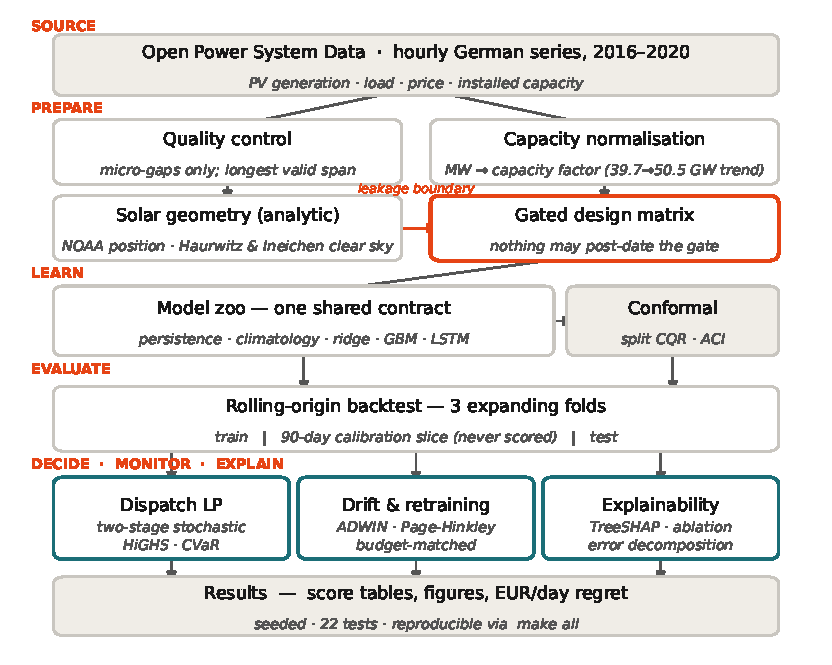
\includegraphics[width=\linewidth]{../figures/pipeline_architecture.pdf}
\caption{The pipeline. The orange boundary is the only structural safety property in the system: everything above it may consume observations freely, and everything at or below it may consume only what existed at gate closure. The three boxes at the bottom consume the same backtest output, which is what allows the forecasting, dispatch, drift and explainability results to be compared without re-running the forecaster three times.}
\label{fig:pipeline}
\end{figure}

\section{Configuration}

Every number a reviewer might want to challenge lives in one dataclass hierarchy mirrored by \texttt{configs/default.yaml}: site coordinates, gate hour, horizon, quantile levels, backtest window lengths, battery energy and power, efficiencies, prices, penalties, CVaR level, scenario count, detector thresholds and retraining budget. No experiment hides a magic number in its body.

\section{Ingestion and features}

The raw package is roughly 130 MB. Ingestion streams it once, selects the German columns by resolving canonical names against a list of candidates so that the code survives an upstream rename, enforces a gap-free hourly index, applies quality control and persists a compact Parquet panel. Feature construction takes 0.1 seconds over the full sample and is cached.

\section{Models and the target-space hook}

Models receive an optional explicit feature subset. This exists for the ablation study in Chapter 5: without it, the ablation would have had to remove columns from the frame, and helper columns re-added for post-processing would have silently re-admitted an ablated family through the back door.

\section{The dispatch linear program}

The commitment and settlement problems are assembled as sparse matrices and solved with HiGHS through \texttt{scipy.optimize.linprog}; no commercial solver is required. A small allocator class assigns contiguous index blocks to each variable family, which keeps the index algebra of a problem with roughly five thousand variables tractable. A forty-scenario commitment solves in about 0.16 seconds, so a two-hundred-day study across five policies runs in a few minutes.

\section{Runtime environment}

One environment detail is load-bearing enough to document. On macOS, LightGBM links the Homebrew OpenMP runtime while PyTorch ships its own. With more than one thread and both runtimes live in a single process, fitting a LightGBM model and then training a torch model \emph{deadlocks}: the process stops with no exception, no traceback and no output. The forecasting experiment fits both. Importing the package therefore pins \texttt{OMP\_NUM\_THREADS} to 1 before any library loads, which was verified to be the only safe setting; two and four both deadlock. The cost is small, because LightGBM parallelises poorly on a design matrix of this shape.

\section{Reproducibility and quality gates}

The suite contains twenty-two tests in three groups.

\textbf{Leakage.} The central test builds the design matrix twice: once on clean data, and once on data in which every observation after a chosen gate has been replaced with a poison value. It then asserts that every row whose origin precedes that gate is bit-for-bit identical between the two matrices. A feature that reached past its gate would pick up the poison and shift. Companion tests assert the horizon band matches the protocol for several gate hours and that every delivery day contributes exactly twenty-four rows.

\textbf{Dispatch economics.} Property tests rather than code-path tests: no forecast-driven policy may beat the perfect-foresight oracle; a perfect forecast must reproduce the oracle cost exactly and incur zero imbalance; state-of-charge dynamics and power limits must hold in settlement; and the asymmetric penalties must push the stochastic commitment above the point commitment.

\textbf{Scoring rules and detectors.} The pinball loss must be minimised at the true quantile; CRPS must be zero for a perfect deterministic forecast and must prefer the sharper of two calibrated forecasts; the interval score must punish a lazily wide interval that coverage alone would reward; the finite-sample conformal correction must not under-cover on a small calibration set; and the drift detectors must produce \emph{identical} event indices on the same shift presented at magnitudes 10 and 0.02.

All randomness is seeded. The full pipeline runs end to end in approximately thirty minutes on a laptop via \texttt{make all}.


\chapter{Results}

\section{Forecasting skill and interval validity (RQ1)}

Fold-averaged over three rolling folds, daylight hours only. PICP is the empirical coverage of the nominal 90 percent interval, PINAW its normalised width, and Winkler the interval score at the same level. Skill is relative to seasonal persistence on MAE.

\par\medskip
\begingroup
\small\setlength{\tabcolsep}{5pt}
\begin{tabular}{@{}llrrrrrr@{}}
\toprule
\textbf{Model} & \textbf{Variant} & \textbf{CRPS} & \textbf{MAE} & \textbf{PICP} & \textbf{PINAW} & \textbf{Winkler} & \textbf{Skill} \\
\midrule
ridge & raw & \textbf{0.0304} & \textbf{0.0444} & 0.846 & 0.784 & 0.243 & +9.9\% \\
ridge & cqr & 0.0307 & 0.0444 & 0.826 & 0.734 & 0.251 & +9.9\% \\
gbm\_quantile & cqr & 0.0313 & 0.0458 & 0.813 & 0.673 & \textbf{0.244} & +7.0\% \\
gbm\_quantile\_k & cqr & 0.0319 & 0.0465 & 0.757 & 0.651 & 0.254 & +5.5\% \\
gbm\_quantile & raw & 0.0328 & 0.0458 & 0.695 & 0.528 & 0.295 & +7.0\% \\
lstm\_quantile & cqr & 0.0332 & 0.0486 & 0.872 & 0.971 & 0.285 & +1.3\% \\
persistence & raw & 0.0334 & 0.0492 & 0.856 & 0.911 & 0.283 & 0.0\% \\
persistence & cqr & 0.0336 & 0.0492 & 0.834 & 0.834 & 0.289 & 0.0\% \\
lstm\_quantile & raw & 0.0342 & 0.0486 & 0.713 & 0.582 & 0.348 & +1.3\% \\
gbm\_quantile\_k & raw & 0.0342 & 0.0465 & 0.582 & 0.437 & 0.342 & +5.5\% \\
gbm\_point\_xgb & cqr & 0.0346 & 0.0481 & 0.650 & 0.618 & 0.335 & +2.3\% \\
gbm\_point & cqr & 0.0348 & 0.0481 & 0.630 & 0.598 & 0.349 & +2.3\% \\
climatology & raw & 0.0356 & 0.0543 & 0.826 & 0.842 & 0.270 & $-$10.1\% \\
climatology & cqr & 0.0358 & 0.0543 & 0.813 & 0.816 & 0.275 & $-$10.1\% \\
climatology\_quantiles & raw & 0.0372 & 0.0571 & 0.856 & 0.914 & 0.257 & $-$15.9\% \\
climatology\_quantiles & cqr & 0.0374 & 0.0571 & 0.877 & 0.973 & 0.259 & $-$15.9\% \\
gbm\_point\_xgb & raw & 0.0402 & 0.0481 & 0.291 & 0.140 & 0.728 & +2.3\% \\
gbm\_point & raw & 0.0413 & 0.0481 & 0.225 & 0.089 & 0.806 & +2.3\% \\
prophet & cqr & 0.0468 & 0.0789 & 0.880 & 1.202 & 0.303 & $-$60.4\% \\
prophet & raw & 0.0469 & 0.0789 & 0.865 & 1.161 & 0.303 & $-$60.4\% \\
\bottomrule
\end{tabular}
\endgroup
\par\medskip

\begin{figure}[H]
\centering
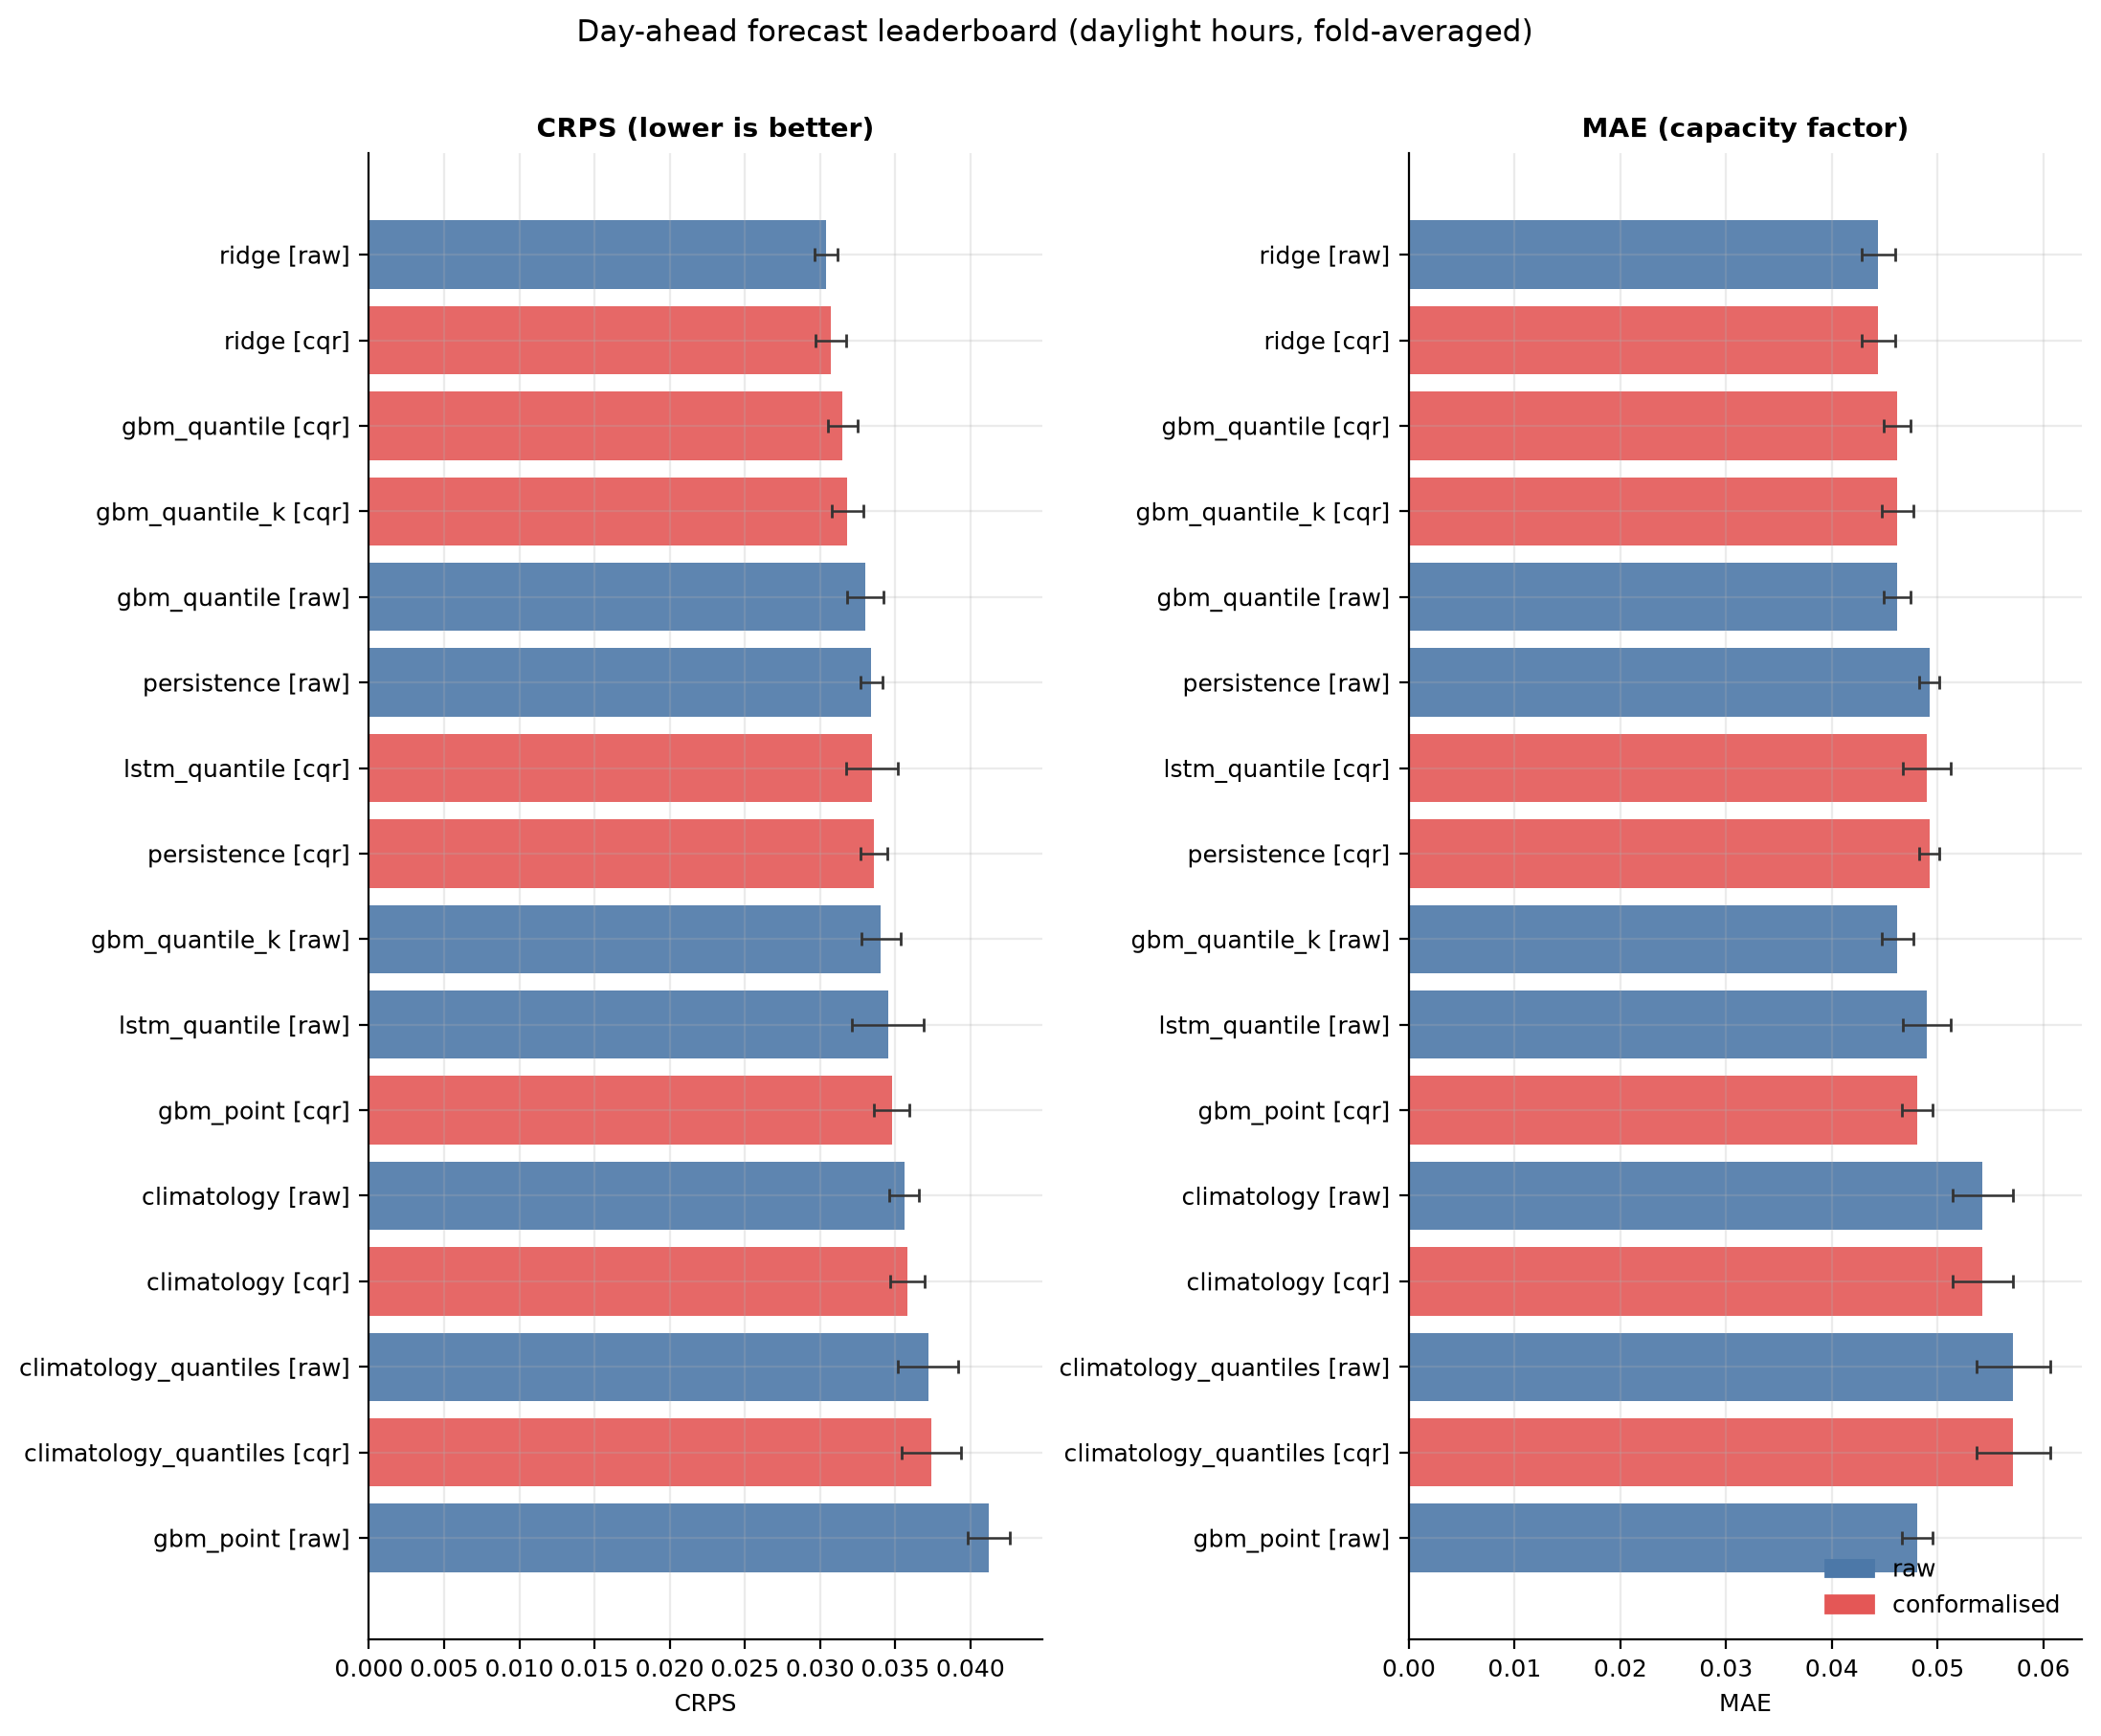
\includegraphics[width=\linewidth]{../figures/02_leaderboard.png}
\caption{The full leaderboard on both a probabilistic and a deterministic score, with fold-to-fold standard errors. Blue bars are raw model output, red bars the same model after split-conformal calibration. The error bars are the reason Section 6.1 describes the top of the table as a cluster rather than a ranking.}
\label{fig:leaderboard}
\end{figure}

\subsection*{Raw quantile intervals are sharp but invalid}

The \texttt{gbm\_point} row is the clearest single result in the study. Its intervals are constructed from in-sample residuals, which the boosted trees have largely fitted away, so a nominal 90 percent interval covers \textbf{22.5 percent} of outcomes. It is simultaneously the sharpest configuration in the table (PINAW 0.089) and by a wide margin the worst, and no metric other than the interval score registers the failure. This is the concrete reason that coverage is never reported here without a Winkler score beside it.

\par\medskip
\begingroup
\small\setlength{\tabcolsep}{7pt}
\begin{tabular}{@{}lrrrrr@{}}
\toprule
\textbf{Model} & \textbf{PICP raw} & \textbf{PICP cqr} & \textbf{Winkler raw} & \textbf{Winkler cqr} & \textbf{Change} \\
\midrule
gbm\_point & 0.225 & 0.630 & 0.806 & 0.349 & $-$57\% \\
gbm\_point\_xgb & 0.291 & 0.650 & 0.728 & 0.335 & $-$54\% \\
gbm\_quantile\_k & 0.582 & 0.757 & 0.342 & 0.254 & $-$26\% \\
lstm\_quantile & 0.713 & 0.872 & 0.348 & 0.285 & $-$18\% \\
gbm\_quantile & 0.695 & 0.813 & 0.295 & 0.244 & $-$17\% \\
\bottomrule
\end{tabular}
\endgroup
\par\medskip
Conformal calibration improves the interval score of every quantile-capable model, and does so by moving coverage toward nominal rather than by widening indiscriminately.

\begin{figure}[H]
\centering
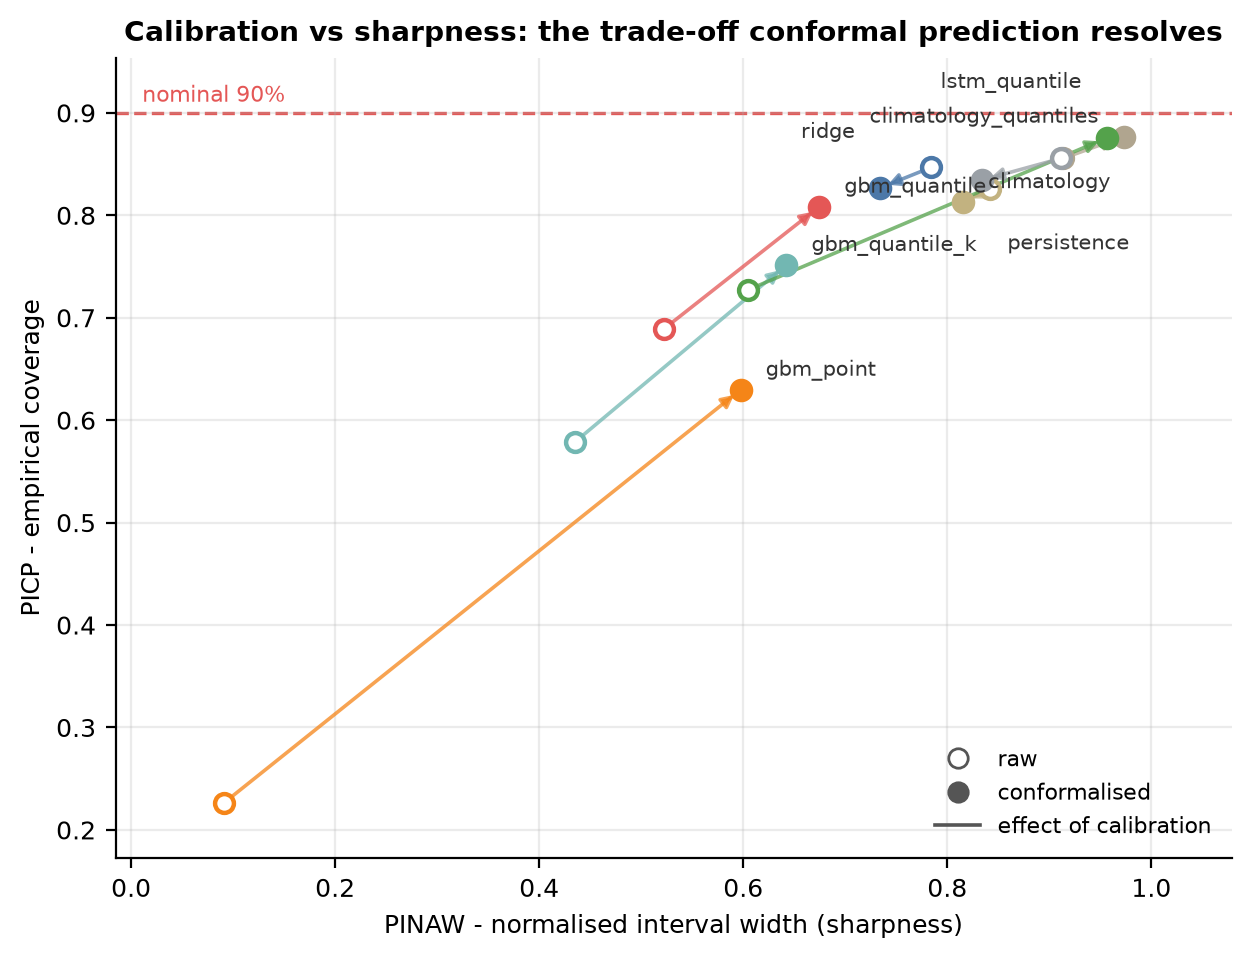
\includegraphics[width=\linewidth]{../figures/04_coverage_vs_width.png}
\caption{Coverage against width. Calibration moves every model upward toward the nominal line at a modest cost in sharpness. A model in the lower left of this plot is not a sharp model; it is a wrong one.}
\label{fig:coverage}
\end{figure}

\begin{figure}[H]
\centering
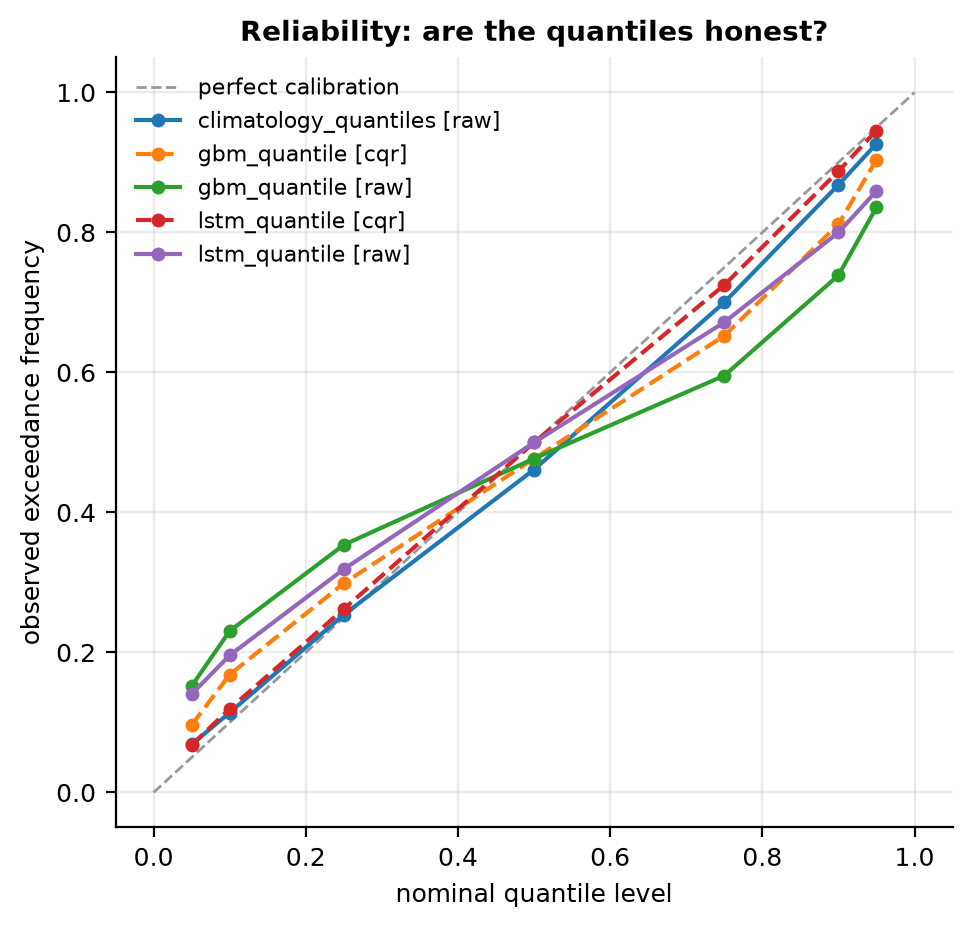
\includegraphics[width=\linewidth]{../figures/03_reliability.png}
\caption{Reliability. Nominal quantile level against observed exceedance frequency; a perfectly calibrated forecaster lies on the diagonal. Deviation below the diagonal in the upper tail is the signature of intervals that are too narrow.}
\label{fig:reliability}
\end{figure}

\subsection*{What the two added baselines settle}

Two rows in the table exist to answer questions the brief raises rather than to compete for the top.

\textbf{Prophet is last, by a wide margin}: CRPS 0.0468 against persistence's 0.0334, and a skill of $-$60 percent. This is the expected result and it is worth having in writing. Prophet is univariate: it sees the timestamp and the history, and none of the engineered features. Its day-ahead forecast is therefore its seasonal decomposition, and Section 5.4 shows that the only genuinely irreplaceable information in this problem is the recent cloud state, which Prophet has no way to consume. It is a strong tool applied to a problem whose difficulty lies entirely outside what it models, and its intervals are correspondingly the widest in the study (PINAW 1.20, wider than the persistence baseline's 0.91).

\textbf{The choice of boosting implementation is immaterial.} LightGBM and XGBoost, given the same features and the same hyperparameters, produce identical MAE to four decimal places (0.0481) and CRPS within 0.0011 of each other. Reporting them as separate rows rather than behind a backend flag makes that visible instead of assumed, and it means the earlier finding that Ridge beats the boosted models is not an artefact of one library's defaults.

\subsection*{Calibration does not fully close the gap}

Even after CQR, coverage sits between 0.76 and 0.88 against a 0.90 nominal. This is not a failure of the method but a consequence of its assumption: split conformal guarantees marginal coverage under exchangeability, and a ninety-day calibration slice followed by a twelve-month test period violates exchangeability about as badly as a seasonal series can. Section 5.3 returns to this with the adaptive procedure.

\begin{figure}[H]
\centering
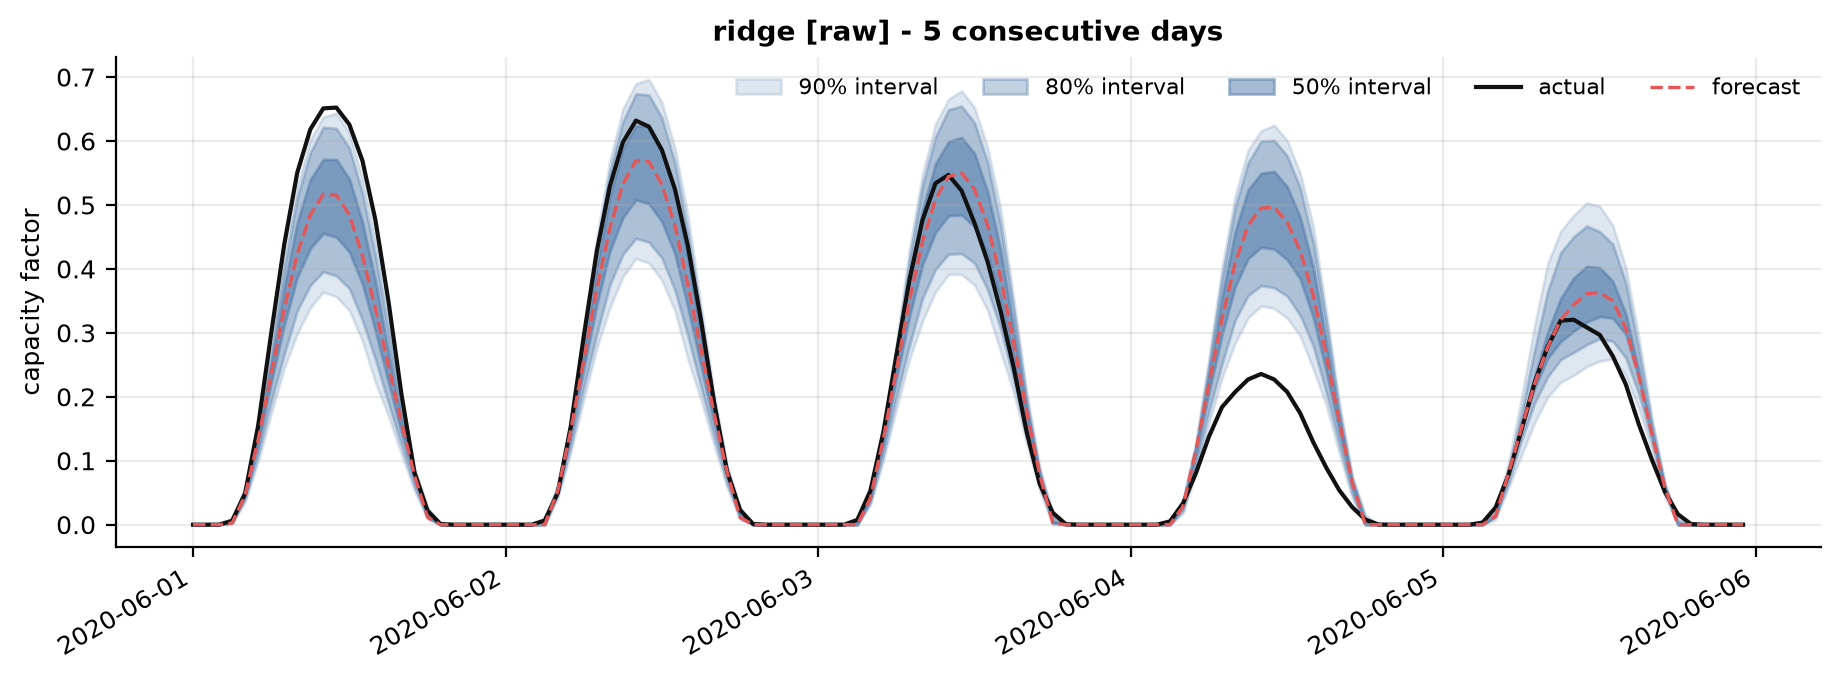
\includegraphics[width=\linewidth]{../figures/05_fan_chart.png}
\caption{The five most variable consecutive delivery days in the test set, with nested 50, 80 and 90 percent intervals. The realised output escapes the 90 percent band twice in five days, on 1 June above and on 4 June below. Two exceedances in five days is visibly worse than the one-in-ten the interval promises, and is the 0.846 marginal coverage of the leading model seen at close range.}
\label{fig:fan}
\end{figure}

\subsection*{Skill, and where the error lives}

Skill against seasonal persistence is approximately 10 percent for the leading configuration. Climatology scores \emph{worse} than persistence, confirming that the exploitable information lies in the recent state of the atmosphere rather than in the seasonal average. The error is highly concentrated: the worst 10 percent of daylight hours carry \textbf{33 percent} of all absolute error, and the worst 25 percent carry 62 percent.

\begin{figure}[H]
\centering
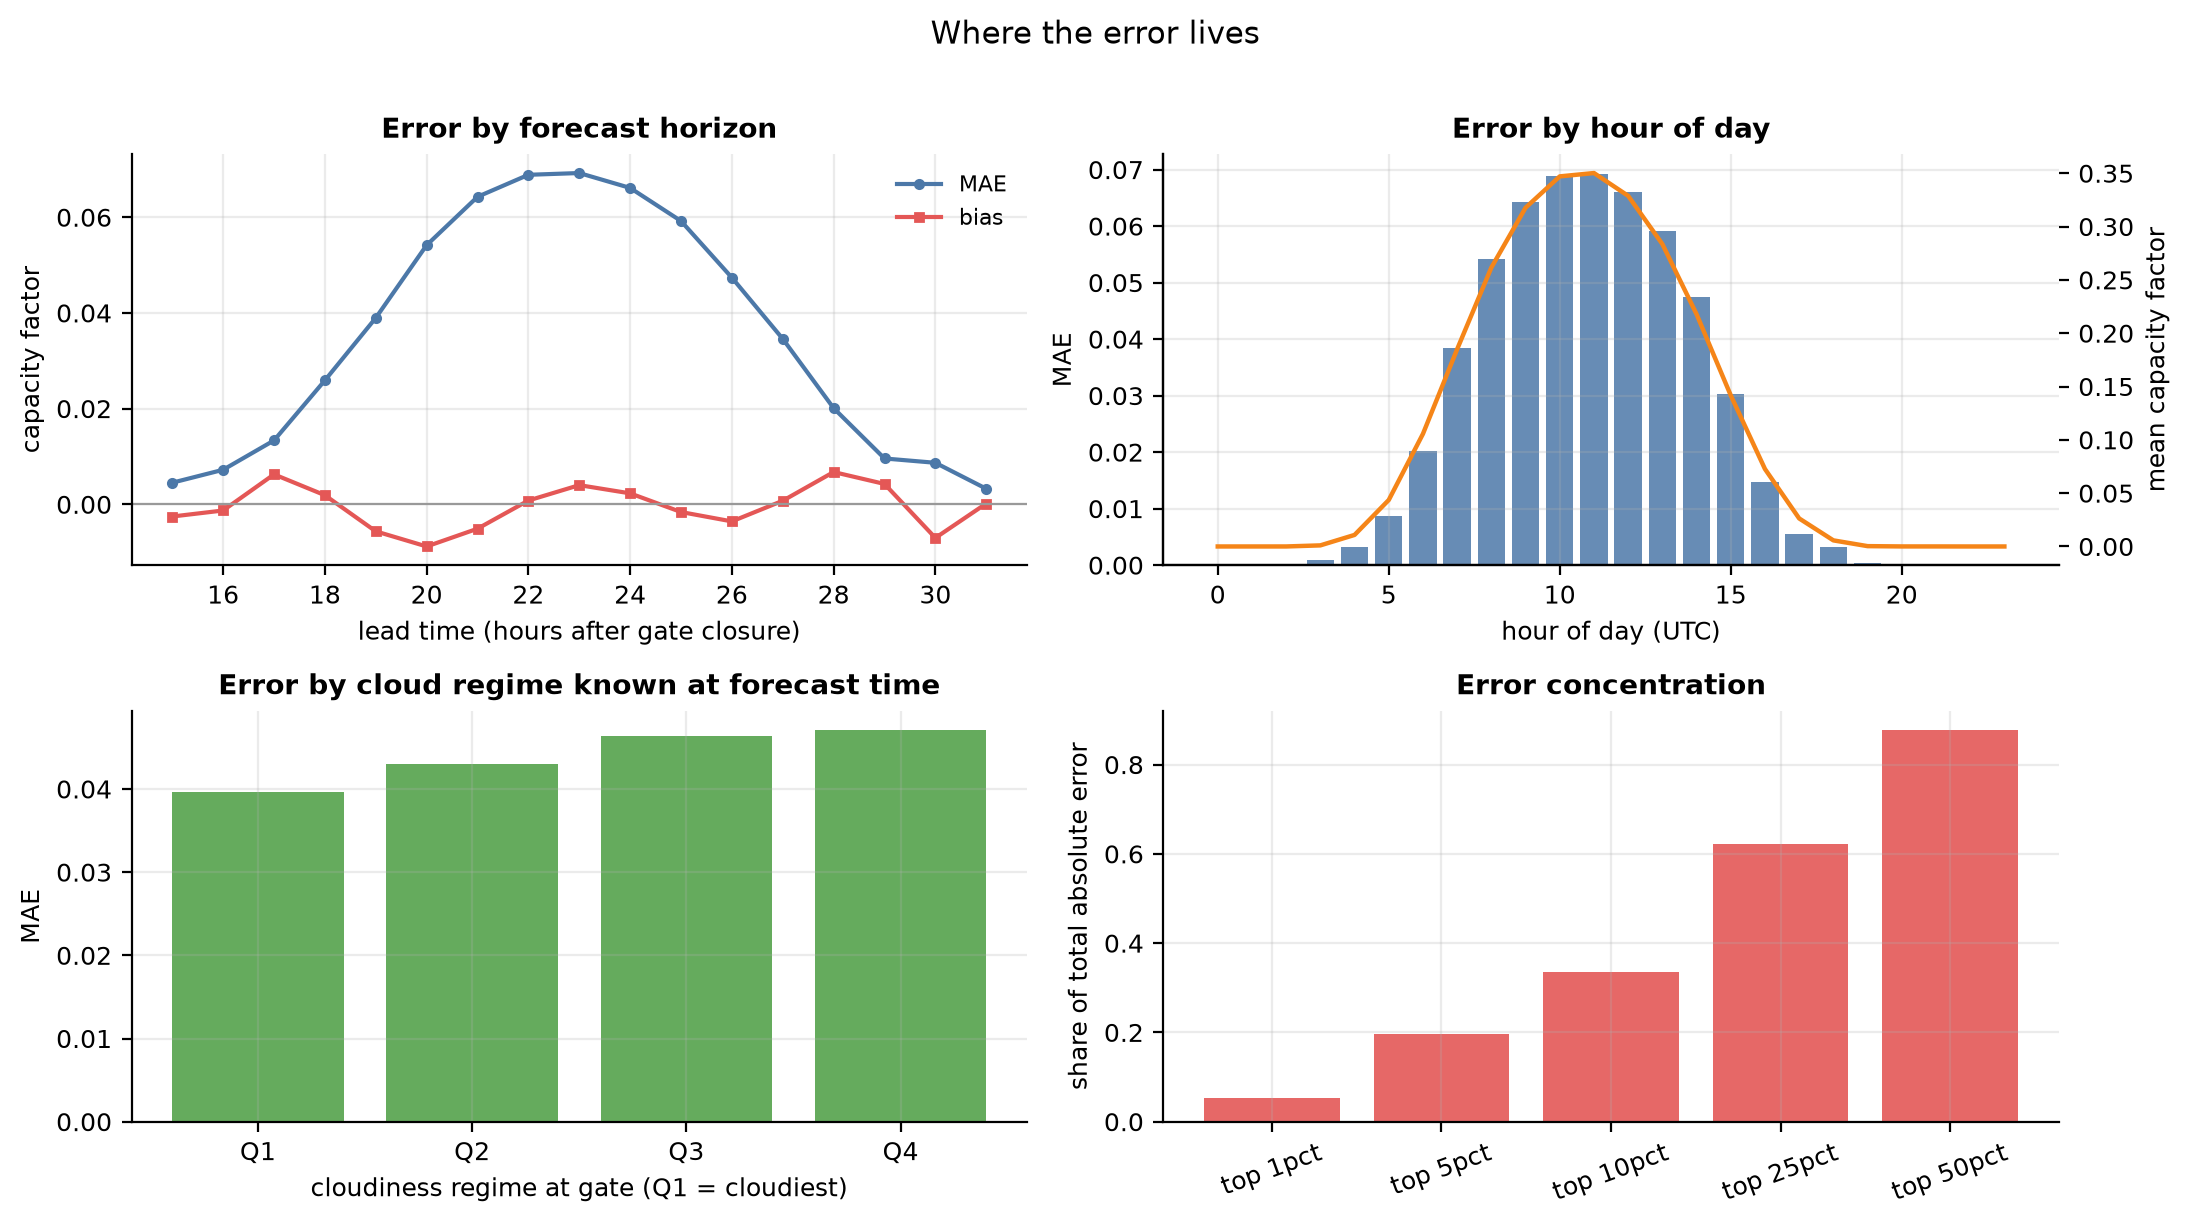
\includegraphics[width=\linewidth]{../figures/06_error_decomposition.png}
\caption{Error decomposition. Error grows only weakly across the 12 to 35 hour horizon band, which is itself a diagnostic of the NWP-free setting: without a weather model, a 13-hour forecast is not much better informed than a 35-hour one. Error rises monotonically from the clearest to the cloudiest regime known at gate closure, confirming that the cloud-state features are being used rather than ignored.}
\label{fig:errordecomp}
\end{figure}

\section{Decision value (RQ2)}

Each delivery day is settled through the two-stage program of Section 3.8. Two hundred delivery days, thinned systematically across seasons so the sample retains the seasonal coverage that random subsampling of a seasonal series would not.

\par\medskip
\begingroup
\small\setlength{\tabcolsep}{6pt}
\begin{tabular}{@{}lrrrrrr@{}}
\toprule
\textbf{Policy} & \textbf{Cost} & \textbf{Regret} & \textbf{p95 regret} & \textbf{Imbalance} & \textbf{Short MWh} & \textbf{vs point} \\
\midrule
oracle & 2180.94 & 0.00 & 0.00 & 0.00 & 0.00 & --- \\
stochastic & 2340.75 & \textbf{159.82} & 454.47 & 146.87 & 0.44 & $-$3.0\% \\
point & 2345.64 & 164.71 & 448.91 & 152.54 & 0.45 & 0.0\% \\
cvar & 2379.36 & 198.43 & 522.18 & 99.27 & 0.21 & +20.5\% \\
quantile ($q$=0.25) & 2388.69 & 207.75 & 507.20 & 103.11 & 0.22 & +26.1\% \\
\bottomrule
\end{tabular}
\endgroup
\par\medskip
All figures are euros per delivery day; regret is measured against the oracle on the same day.

At the baseline parameters the advantage of the stochastic policy over the point policy is small: 3.0 percent of regret. The two risk-averse policies perform \emph{worse} than the point forecast. Both roughly halve the energy shortfall, from 0.45 to about 0.21 MWh per day, but they pay more for that reduction in the day-ahead market than the imbalance penalty they avoid. A study that reported only the reduction in imbalance volume would have concluded the opposite.

\begin{figure}[H]
\centering
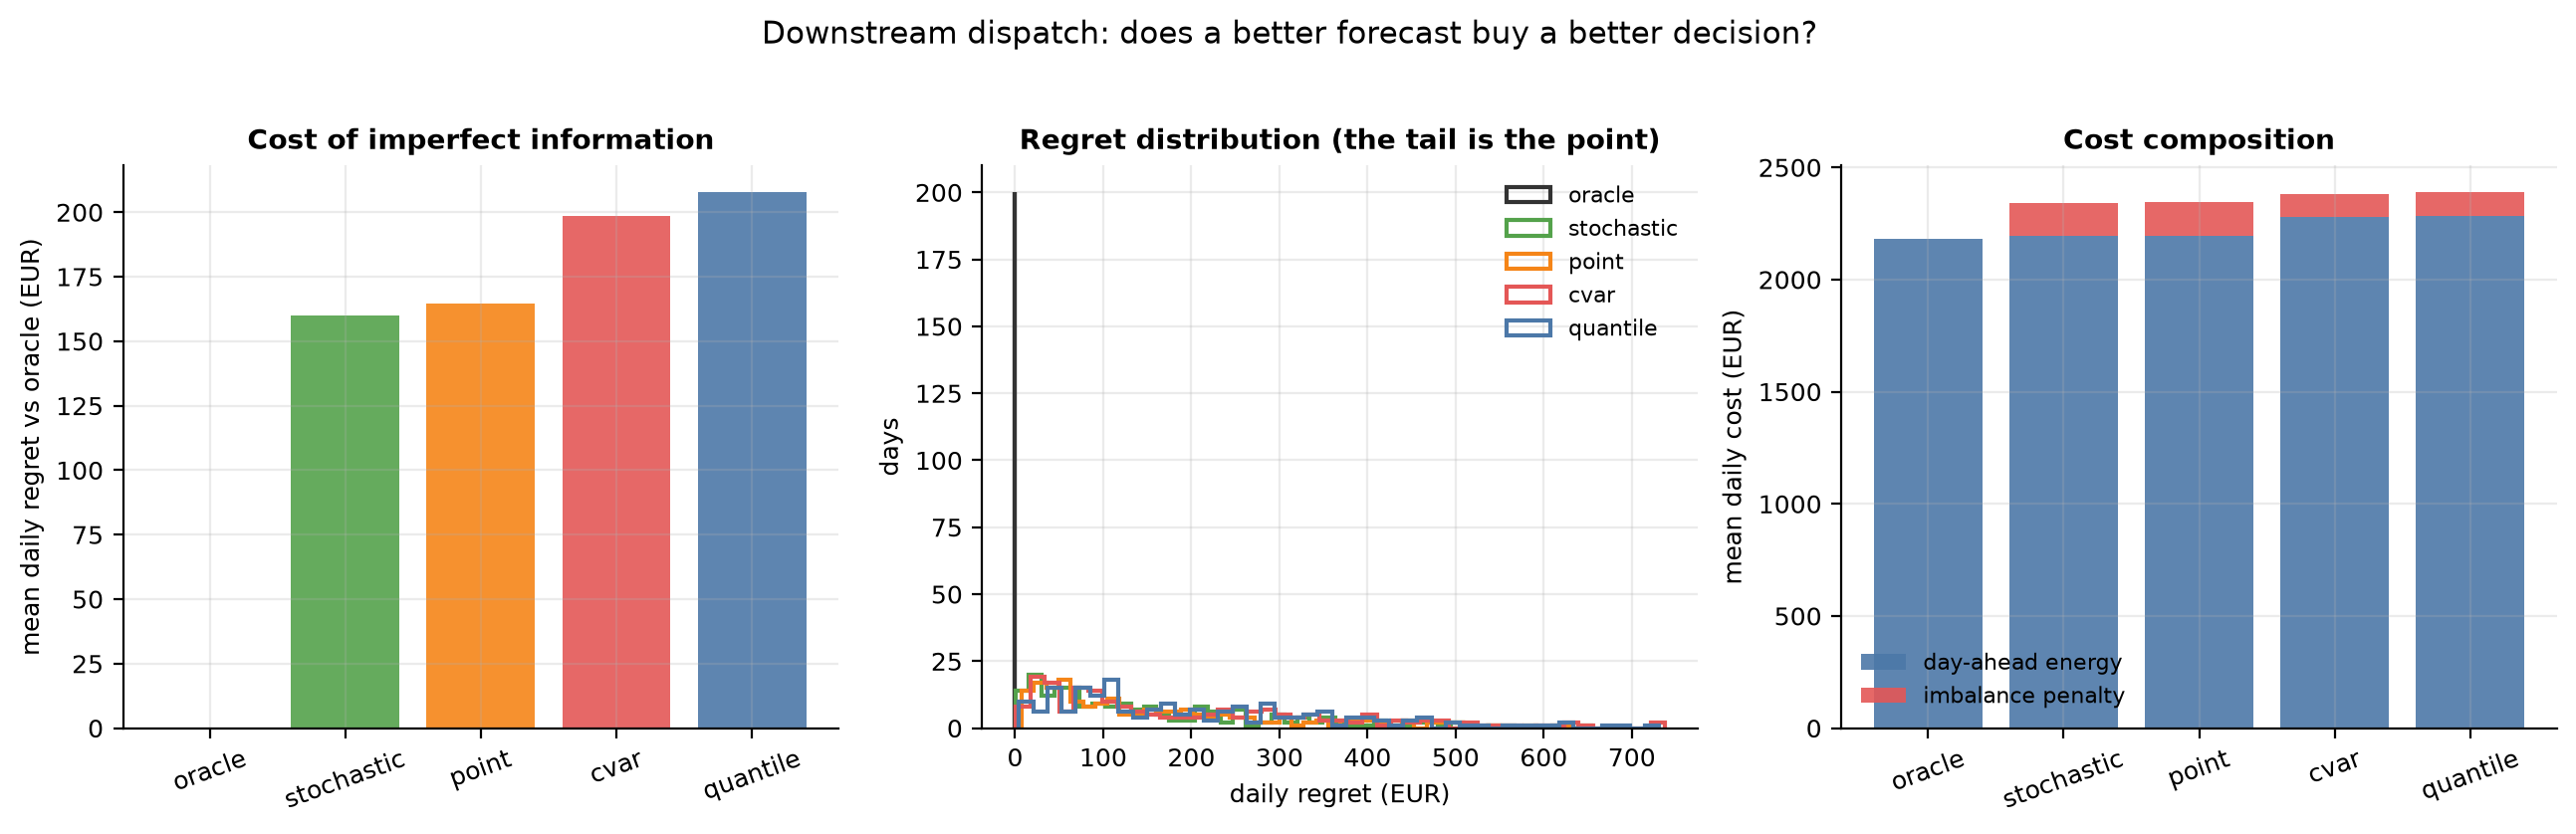
\includegraphics[width=\linewidth]{../figures/07_dispatch.png}
\caption{Dispatch outcomes by policy. The middle panel carries the operational content: the distributions overlap heavily in the body and separate in the tail, and it is the tail that determines whether a month is profitable.}
\label{fig:dispatch}
\end{figure}

\subsection*{Which quantile should be committed to}

Sweeping the fixed commitment quantile produces a clean U-shaped regret curve with a minimum at $q = 0.55$ and a regret of 149.06 euros per day, better than any of the five policies above. The newsvendor critical fractile implied by the penalty asymmetry is 0.667.

\par\medskip
\begingroup
\small\setlength{\tabcolsep}{8pt}
\begin{tabular}{@{}lrrrrrrrrrr@{}}
\toprule
\textbf{Quantile} & 0.05 & 0.15 & 0.25 & 0.35 & 0.45 & \textbf{0.55} & 0.65 & 0.75 & 0.85 & 0.95 \\
\midrule
\textbf{Regret} & 422 & 270 & 193 & 169 & 154 & \textbf{149} & 161 & 183 & 240 & 352 \\
\bottomrule
\end{tabular}
\endgroup
\par\medskip

\begin{figure}[H]
\centering
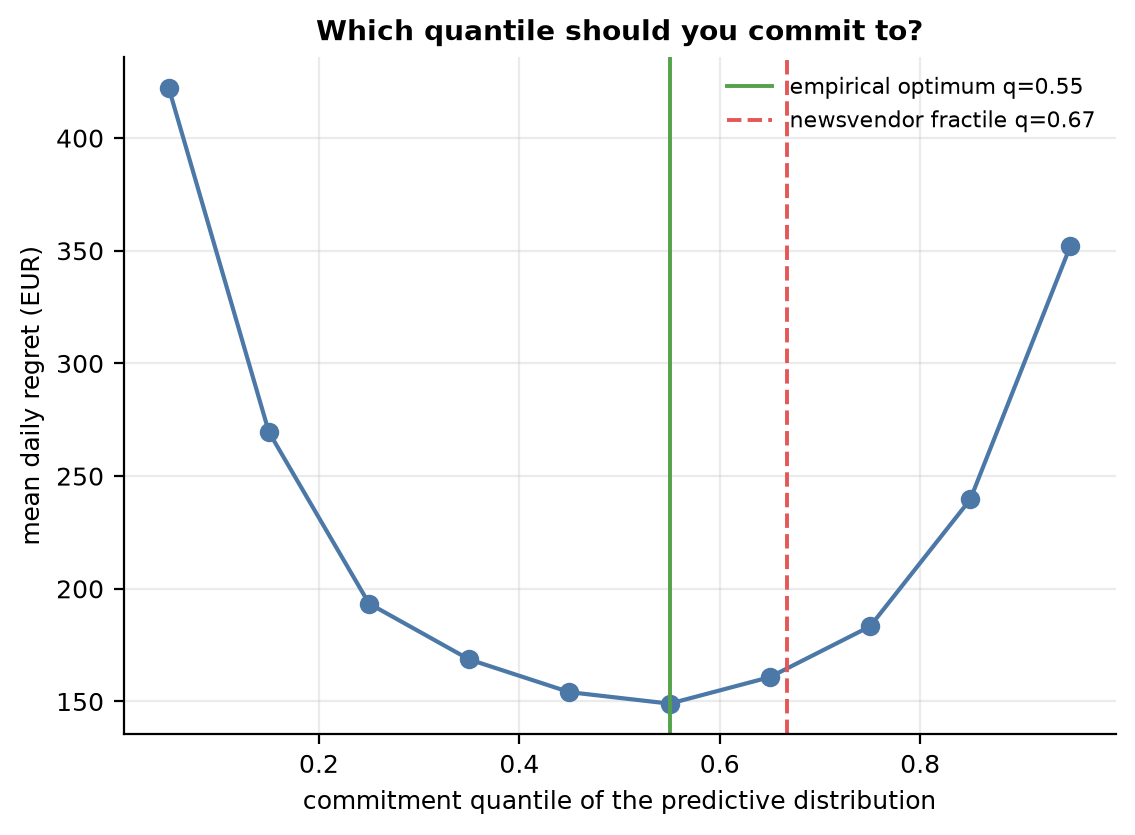
\includegraphics[width=\linewidth]{../figures/11_quantile_sweep.png}
\caption{Regret against commitment quantile. The empirical optimum sits below the newsvendor fractile. The classical newsvendor has no recourse, whereas this operator has a battery that absorbs after the fact exactly the shortfall a conservative commitment would have hedged in advance, so part of the newsvendor premium has already been paid for in hardware.}
\label{fig:sweep}
\end{figure}

\subsection*{Forecast score against decision cost}

Across all twenty model and variant combinations, CRPS and mean dispatch regret correlate at $r = 0.884$.

That figure is higher than the same correlation before Prophet joined the comparison, and the reason is worth stating rather than quietly banking. Prophet is both much the worst forecast (CRPS 0.0468) and much the most expensive decision (267 euros per day against the best model's 144), so adding it stretches the range on both axes and mechanically raises the correlation. A correlation computed over a set of models the analyst chose is a property of that set as much as of the underlying relationship; quoting it without saying which models were in the set overstates how safely a scoring rule stands in for a cost.

Within the set, the relationship is still loose enough to invert on individual pairs. \texttt{gbm\_quantile\_k[raw]} has a clearly worse CRPS than its conformalised counterpart (0.0341 against 0.0318, a seven percent difference) and yet a slightly \emph{lower} dispatch regret (161.74 against 162.13 euros per day). The same inversion appears at the top of the table: \texttt{ridge[cqr]} scores worse on CRPS than \texttt{ridge[raw]} (0.0305 against 0.0302) and is cheaper to act on (144.32 against 144.82).

\begin{figure}[H]
\centering
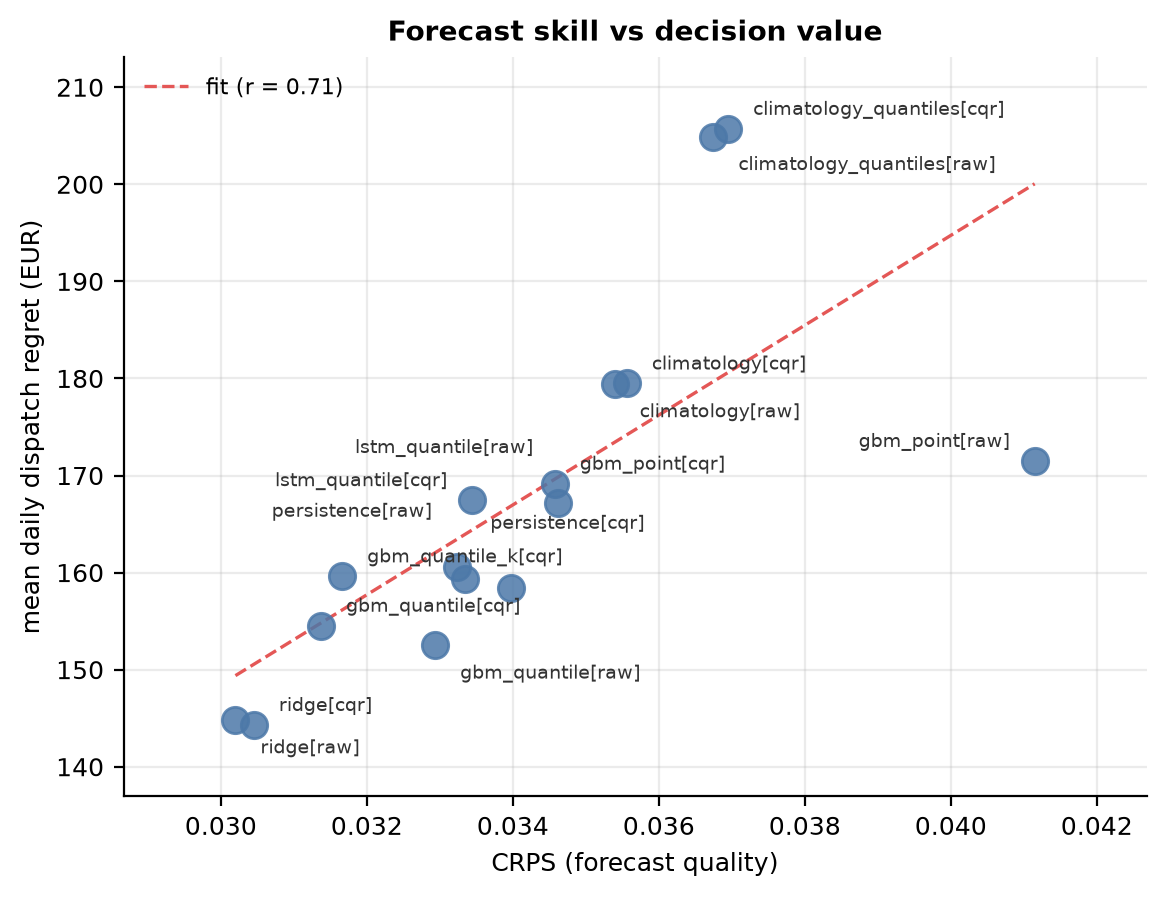
\includegraphics[width=\linewidth]{../figures/08_forecast_vs_decision.png}
\caption{Forecast quality against decision value for all twenty configurations. Ranking models by a proper scoring rule and ranking them by money are correlated exercises, not identical ones.}
\label{fig:value}
\end{figure}

\subsection*{When the predictive distribution is worth having}

The 3 percent headline is not a property of probabilistic forecasting. It is a property of probabilistic forecasting at one imbalance penalty and one battery size. Sweeping both, at ninety delivery days per cell:

\par\medskip
\begingroup
\small\setlength{\tabcolsep}{9pt}
\begin{tabular}{@{}lrrrr@{}}
\toprule
\textbf{Imbalance penalty (EUR/MWh)} & \textbf{0 MWh} & \textbf{2 MWh} & \textbf{4 MWh} & \textbf{8 MWh} \\
\midrule
150 & +46.7\% & +67.5\% & +64.7\% & +59.8\% \\
300 (baseline) & +17.0\% & +8.6\% & +6.4\% & +8.3\% \\
600 & +2.7\% & +4.0\% & +10.5\% & +16.1\% \\
1200 & +17.8\% & +22.4\% & +29.8\% & +35.2\% \\
\bottomrule
\end{tabular}
\endgroup
\par\medskip
Values are the percentage reduction in regret achieved by the stochastic policy relative to the point policy.

\begin{figure}[H]
\centering
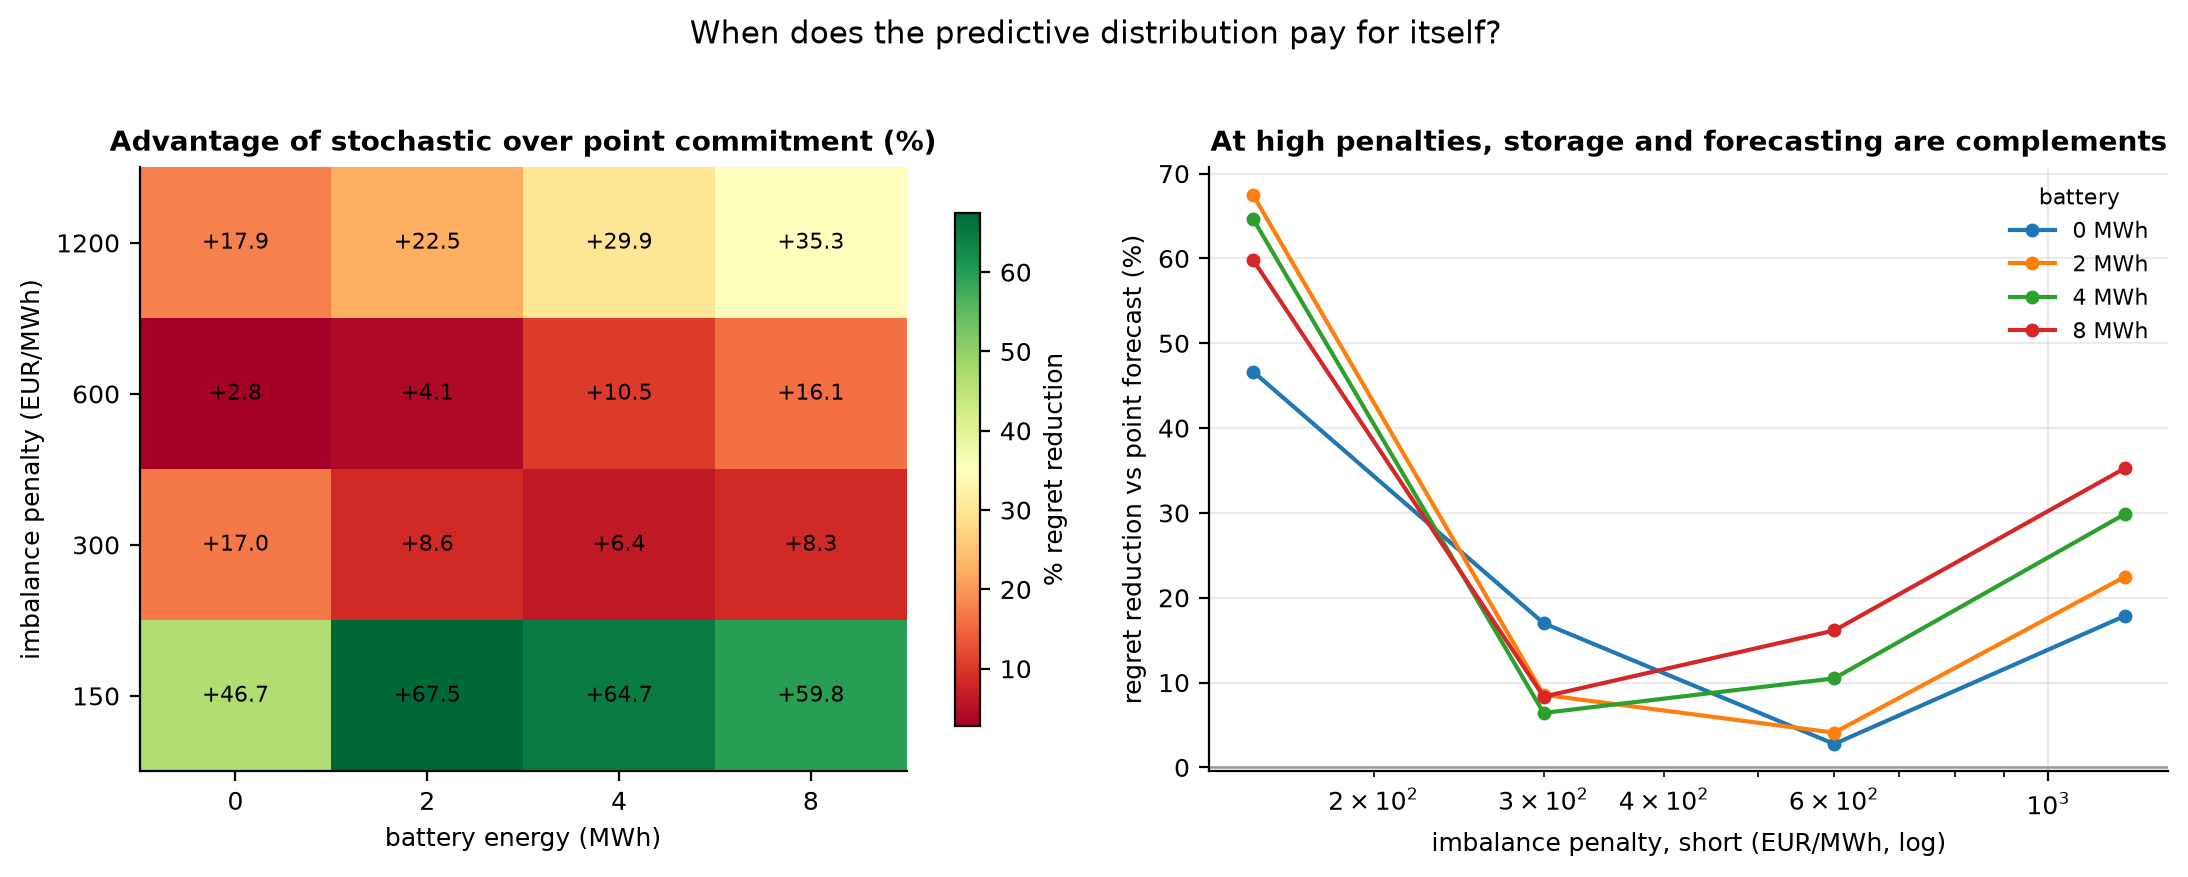
\includegraphics[width=\linewidth]{../figures/13_sensitivity.png}
\caption{The value of the predictive distribution across the penalty and storage grid. It ranges from 3 to 67 percent, which is why no single ``probabilistic beats point'' number is meaningful without stating the penalty regime and the flexibility available.}
\label{fig:sensitivity}
\end{figure}

\section{Concept drift and retraining (RQ3)}

Population stability index and Kolmogorov-Smirnov statistics computed on the \emph{inputs} between the early and late halves of the sample flag 3 of 55 features above the conventional PSI threshold of 0.2. Because these are input-side diagnostics they would fire even where labels arrive with a delay, which is the usual operational situation.

Three retraining policies, simulated day by day over a two-year test period at a matched budget of six refits:

\par\medskip
\begingroup
\small\setlength{\tabcolsep}{8pt}
\begin{tabular}{@{}lrrrrrr@{}}
\toprule
\textbf{Policy} & \textbf{MAE} & \textbf{RMSE} & \textbf{CRPS} & \textbf{PICP} & \textbf{Refits} & \textbf{Triggers} \\
\midrule
static (never refit) & 0.0439 & 0.0649 & 0.0304 & 0.924 & 1 & 0 \\
periodic (calendar) & 0.0437 & 0.0642 & 0.0301 & 0.887 & 7 & 0 \\
drift-triggered & \textbf{0.0434} & \textbf{0.0639} & \textbf{0.0301} & 0.892 & \textbf{2} & 1 \\
\bottomrule
\end{tabular}
\endgroup
\par\medskip
Drift-triggered retraining attains the best value on every accuracy metric while spending two refits against the calendar policy's seven. The accuracy margin is small in absolute terms; the difference in retraining spend is not.

\begin{figure}[H]
\centering
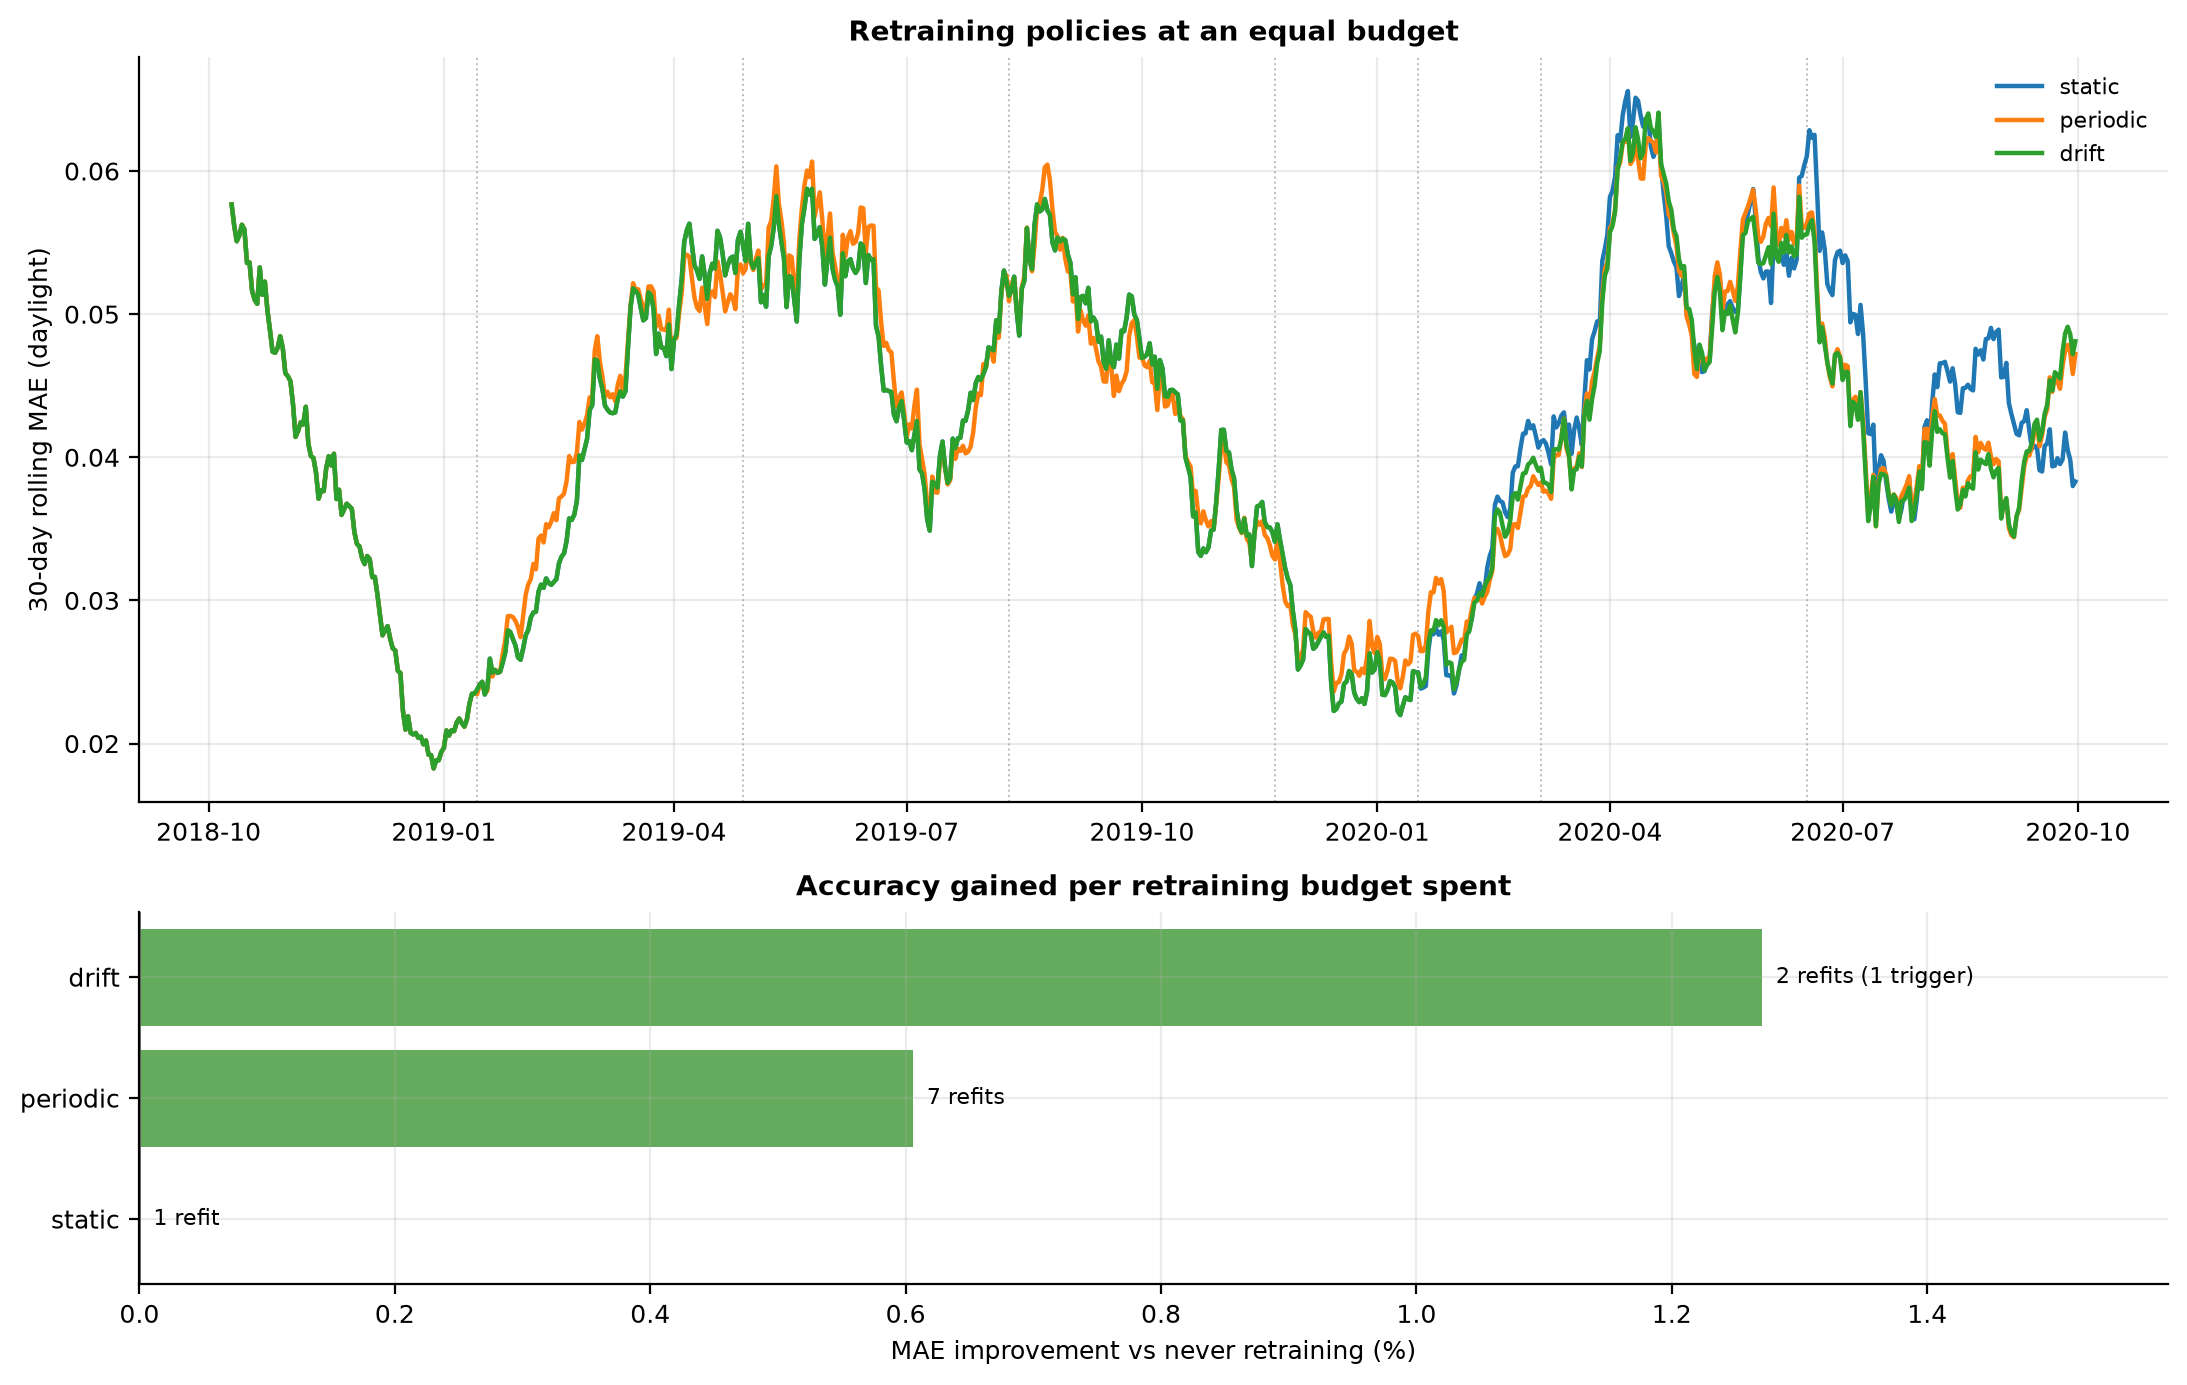
\includegraphics[width=\linewidth]{../figures/09_drift.png}
\caption{Retraining policies at an equal budget. The seasonal cycle dominates the error trajectory and the three policies track one another closely for most of the period, separating in the second winter. The lower panel plots improvement relative to never retraining rather than absolute MAE, because on a zero-based axis 0.0434 and 0.0439 are indistinguishable and the result would be invisible.}
\label{fig:drift}
\end{figure}

\subsection*{The detectors had to be fixed before this question could be answered}

On the first run every detector reported \textbf{zero} triggers, which made RQ3 unanswerable rather than answered in the negative. The cause is that ADWIN and Page-Hinkley threshold \emph{absolute} deviations, while the daily mean-error stream has a magnitude of about 0.04. A direct probe confirmed the diagnosis: the ADWIN implementation used here detects a step from 0 to 10 but does not detect a step from 0.02 to 0.06, a threefold relative change, because the Hoeffding bound it compares against is larger than the entire signal. The Page-Hinkley default threshold of $\lambda = 30$ was roughly three orders of magnitude too large for the same reason.

The fix is to standardise the stream, freezing the mean and variance after a warm-up window so that the normaliser cannot absorb the very shift it is meant to expose. Thresholds then become scale-free, and a regression test asserts that the same shift presented at magnitudes 10 and 0.02 produces identical event indices. With this in place the detected change points are seasonal: ADWIN fires in January, Page-Hinkley in the March-April transition when PV error climbs steeply.

\subsection*{Adaptive conformal inference}

Section 5.1 left split conformal under-covering because seasonality breaks exchangeability. Adapting the miscoverage level online addresses this directly.

\par\medskip
\begingroup
\small\setlength{\tabcolsep}{10pt}
\begin{tabular}{@{}lrrr@{}}
\toprule
\textbf{Method} & \textbf{Coverage} & \textbf{Worst-month coverage} & \textbf{Mean width} \\
\midrule
split conformal ($\gamma = 0$) & 0.903 & 0.828 & 0.1696 \\
adaptive ($\gamma = 0.005$) & 0.900 & 0.857 & 0.1687 \\
adaptive ($\gamma = 0.02$) & 0.900 & 0.874 & 0.1650 \\
adaptive ($\gamma = 0.05$) & 0.896 & \textbf{0.879} & \textbf{0.1606} \\
\bottomrule
\end{tabular}
\endgroup
\par\medskip
Split conformal achieves correct \emph{marginal} coverage, 0.903 against a 0.90 target, while failing \emph{conditionally}: in its worst month it covers 83 percent. Adaptive conformal raises worst-month coverage to 88 percent and is simultaneously \emph{sharper}. Validity here is not purchased with wider intervals; it is purchased by placing the width where it is needed. For an operator exposed to imbalance penalties the worst-month figure is the one that matters, because that is the month in which the penalties arrive.

\begin{figure}[H]
\centering
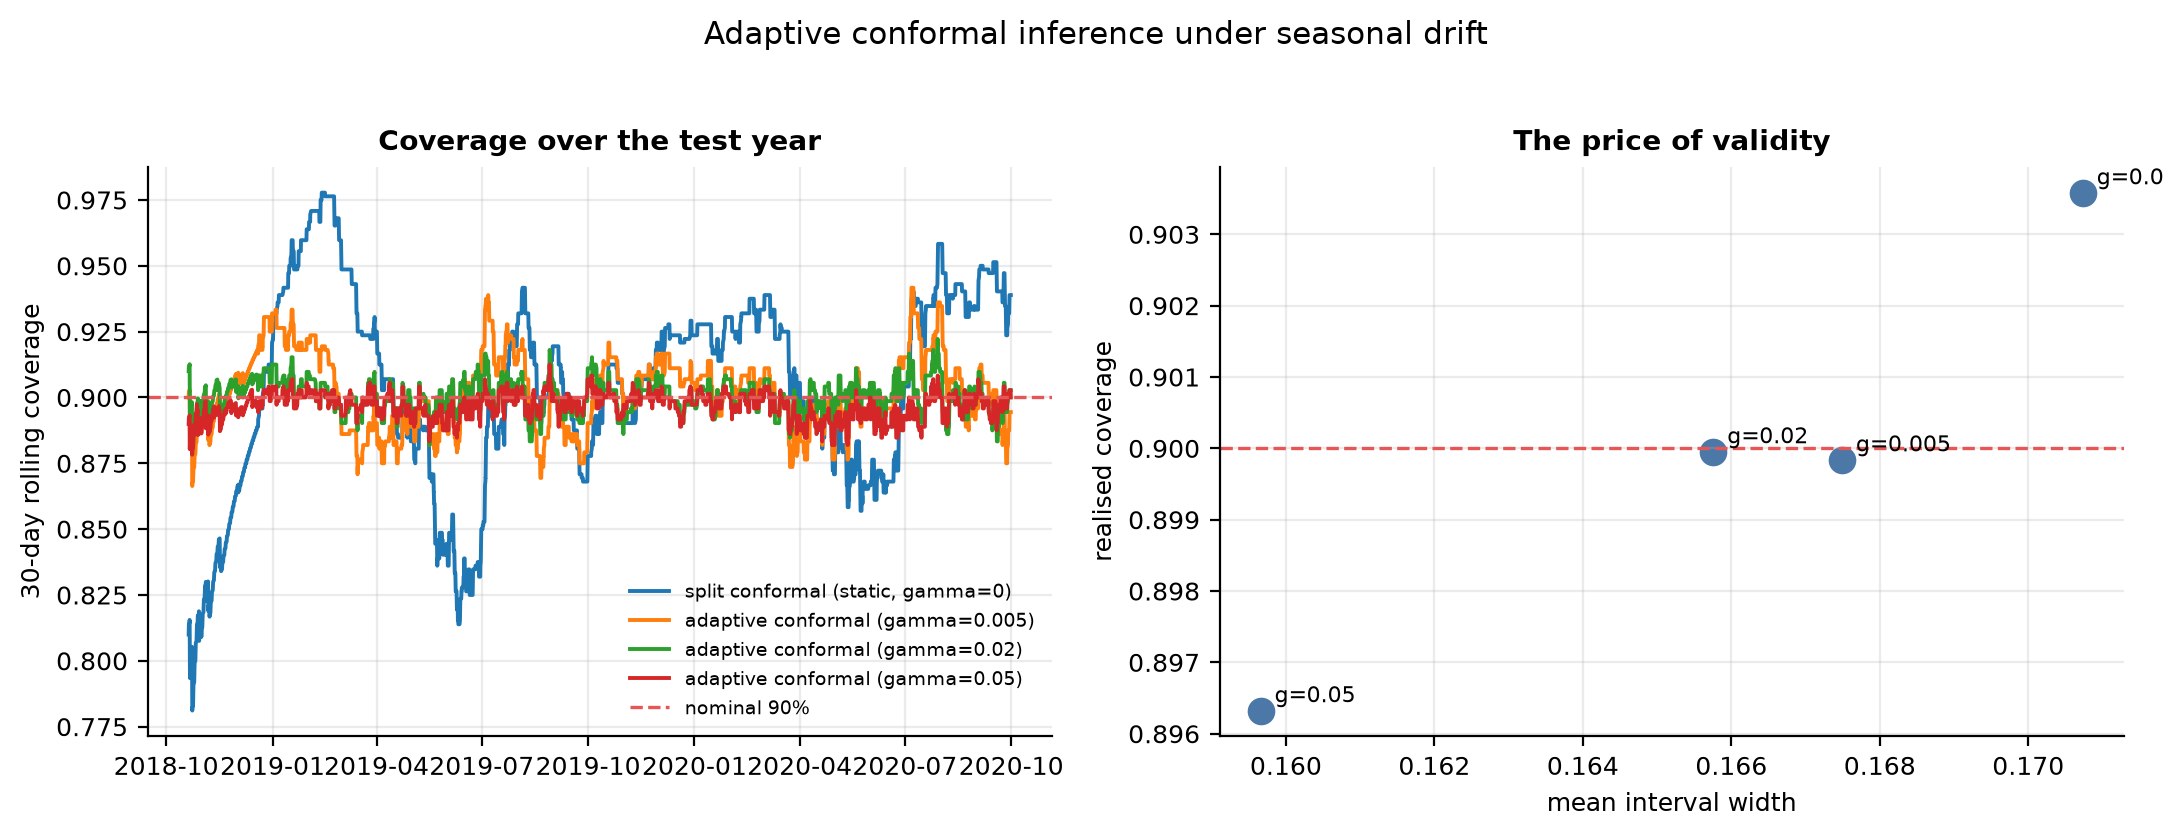
\includegraphics[width=\linewidth]{../figures/12_adaptive_conformal.png}
\caption{Rolling coverage across the test year, and the coverage-width trade-off. The first implementation of the adaptive procedure widened intervals by requesting increasingly extreme quantiles from the fitted grid; because interpolation clamps outside the 0.05 to 0.95 range, the interval could never exceed the model's own 90 percent band, coverage saturated at 0.70, and adaptation appeared actively harmful. The score-based formulation reported here has no such ceiling.}
\label{fig:aci}
\end{figure}

\section{Explainability (RQ4)}

TreeSHAP attribution grouped into feature families, set against leave-one-family-out ablation on the same model and the same test period.

\par\medskip
\begingroup
\small\setlength{\tabcolsep}{10pt}
\begin{tabular}{@{}lrrr@{}}
\toprule
\textbf{Feature family} & \textbf{Share of $|$SHAP$|$} & \textbf{MAE if removed} & \textbf{Change} \\
\midrule
physical (solar geometry) & 67.3\% & 0.0432 & $-$1.6\% \\
autoregressive lags & 17.3\% & 0.0441 & +0.5\% \\
recent state at origin & 8.5\% & 0.0450 & \textbf{+2.6\%} \\
calendar & 3.7\% & 0.0435 & $-$0.8\% \\
exogenous & 3.2\% & 0.0449 & +2.3\% \\
\midrule
full model & --- & 0.0438 & --- \\
\bottomrule
\end{tabular}
\endgroup
\par\medskip

The two rankings disagree almost completely, and the disagreement is the finding. Solar geometry receives two-thirds of all attribution, yet deleting the entire family leaves accuracy very slightly \emph{better}, and the calendar block behaves the same way. The rolling clear-sky-index statistics receive 8.5 percent of attribution but constitute the single most irreplaceable family, and the exogenous block -- 3.2 percent of attribution, the smallest share in the table -- is the second most irreplaceable. The two orderings are close to reversed.

\begin{figure}[H]
\centering
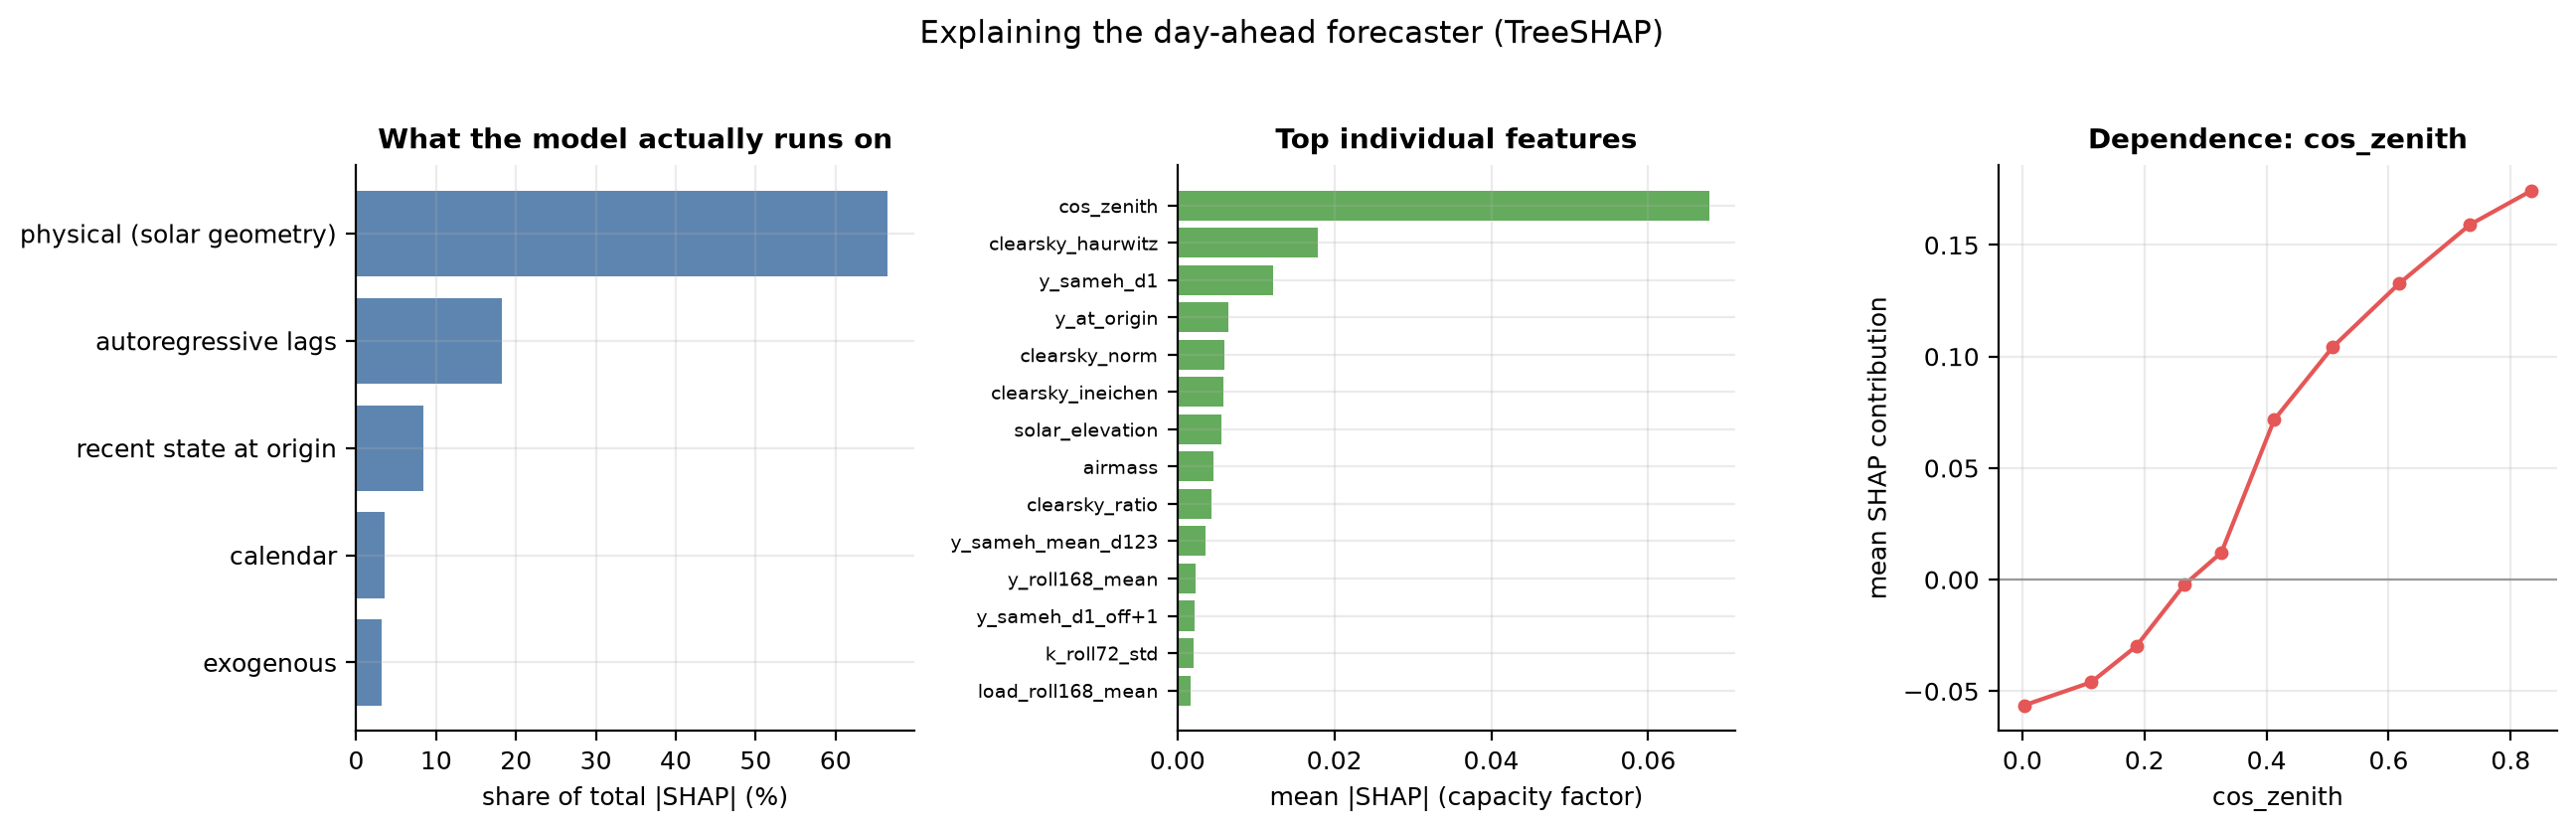
\includegraphics[width=\linewidth]{../figures/10_shap.png}
\caption{TreeSHAP attribution by feature family, the leading individual features, and a dependence curve for the strongest of them. The features whose attributions correlate most strongly with realised error are all clear-sky-index terms and all correlate negatively, meaning the model errs most on the days when it is leaning hardest on recent cloud state.}
\label{fig:shap}
\end{figure}

\section{A small-data strategy for a new site (RQ5)}

Germany is the source. The targets are Switzerland, Denmark and Great Britain, each evaluated on five held-out 60-day windows, with the local-history budget varied from one week to sixteen months. All figures are fold-averaged MAE on the target site's own held-out periods.

\par\medskip
\begingroup
\small\setlength{\tabcolsep}{7pt}
\begin{tabular}{@{}lrrrrrrr@{}}
\toprule
\textbf{Site} & \textbf{Lat.} & \textbf{zero-shot} & \textbf{local 7\,d} & \textbf{local 480\,d} & \textbf{pooled 7\,d} & \textbf{best pooled} & \textbf{crossover} \\
\midrule
Switzerland   & 46.9\textdegree N & 0.1479 & 0.2310 & 0.0652 & \textbf{0.0647} & 0.0608 & 120\,d \\
Denmark       & 56.0\textdegree N & 0.1091 & 0.2696 & 0.0829 & 0.0908 & 0.0766 & 240\,d \\
Great Britain & 51.5\textdegree N & 0.0899 & 0.3729 & 0.0828 & \textbf{0.0823} & 0.0797 & 240\,d \\
\bottomrule
\end{tabular}
\endgroup
\par\medskip

Three results, in increasing order of practical consequence.

\textbf{Zero-shot transfer works, and works well.} A model trained on Germany and applied to Switzerland with no local data at all achieves an MAE of 0.1479, against 0.2310 for a model trained on the target site's own first week. The same holds at all three sites. This is not a trivial outcome: the sites span nine degrees of latitude and quite different climates. It works because the representation is portable by construction --- the target is normalised, and the clear-sky block is recomputed for the target's own coordinates, so what transfers is the relationship between recent atmospheric state and tomorrow's output rather than anything site-specific.

\textbf{Local-only training needs four to eight months of history to catch up.} The crossover is 120 days for Switzerland and 240 days for both Denmark and Great Britain. Below that, an operator training only on local data is worse off than one who simply borrowed a model from another country.

\textbf{Pooling beats both, and beats them immediately.} Training on the source and local data together, with the local rows upweighted, produces the best result at essentially every budget. At Switzerland and Great Britain, pooled training with \emph{seven days} of local history already beats local-only training with \emph{480 days} --- 0.0647 against 0.0652, and 0.0823 against 0.0828. Denmark is the exception: pooled at seven days (0.0908) does not quite reach local-only at 480 days (0.0829), though pooled at its own best budget (0.0766) beats it comfortably.

\begin{figure}[H]
\centering
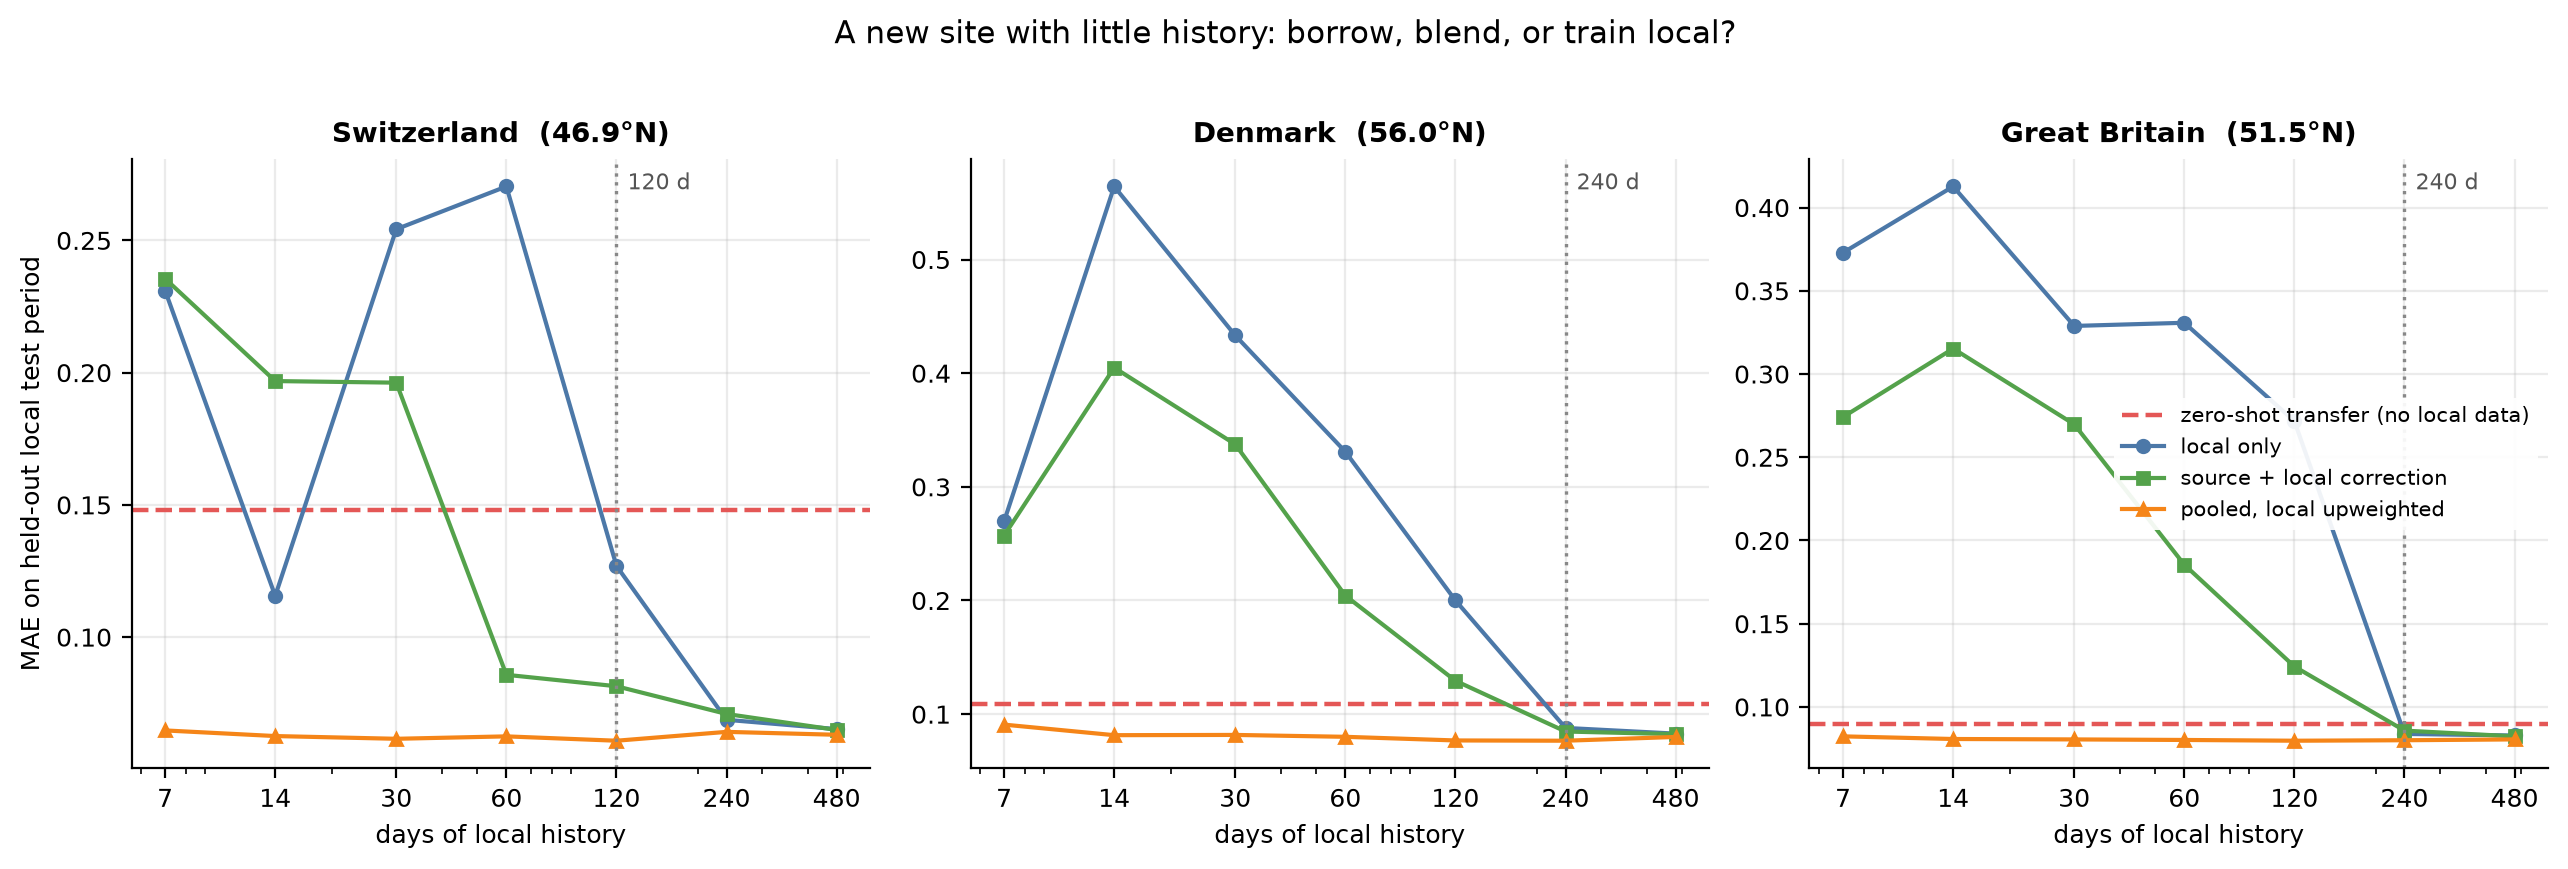
\includegraphics[width=\linewidth]{../figures/14_transfer_curves.png}
\caption{MAE against local training budget at each target site, fold-averaged over five 60-day evaluation windows. The x-axis is logarithmic because the budgets span a factor of nearly seventy and the interesting behaviour is all at the short end. Zero-shot is drawn as a horizontal line because it consumes no local data and therefore has the same value at every budget; its intersection with the local curve is the quantity the experiment exists to measure. The pooled curve is close to flat, which is the finding restated: almost all of its performance comes from the source data, and the local rows only steer it.}
\label{fig:transfer_curves}
\end{figure}

The pooled curve being flat is worth dwelling on. Between seven days and 480 days of local history, pooled MAE at Great Britain moves from 0.0823 to 0.0805 --- a two percent improvement for sixty-eight times the data. Whatever the local rows contribute, they contribute almost all of it in the first week.

\textbf{A short local window is seasonally biased, not merely small.} The local curves are not monotonic even after averaging over five windows: Swiss local-only MAE falls to 0.1156 at fourteen days, rises to 0.2704 at sixty, then falls again. Thirty days of history is one season of history, and a model fitted to it has no way to identify the seasonal terms it will be asked to extrapolate across. This is why the reported crossover requires local training to win \emph{and keep winning}, rather than to win once.

\begin{figure}[H]
\centering
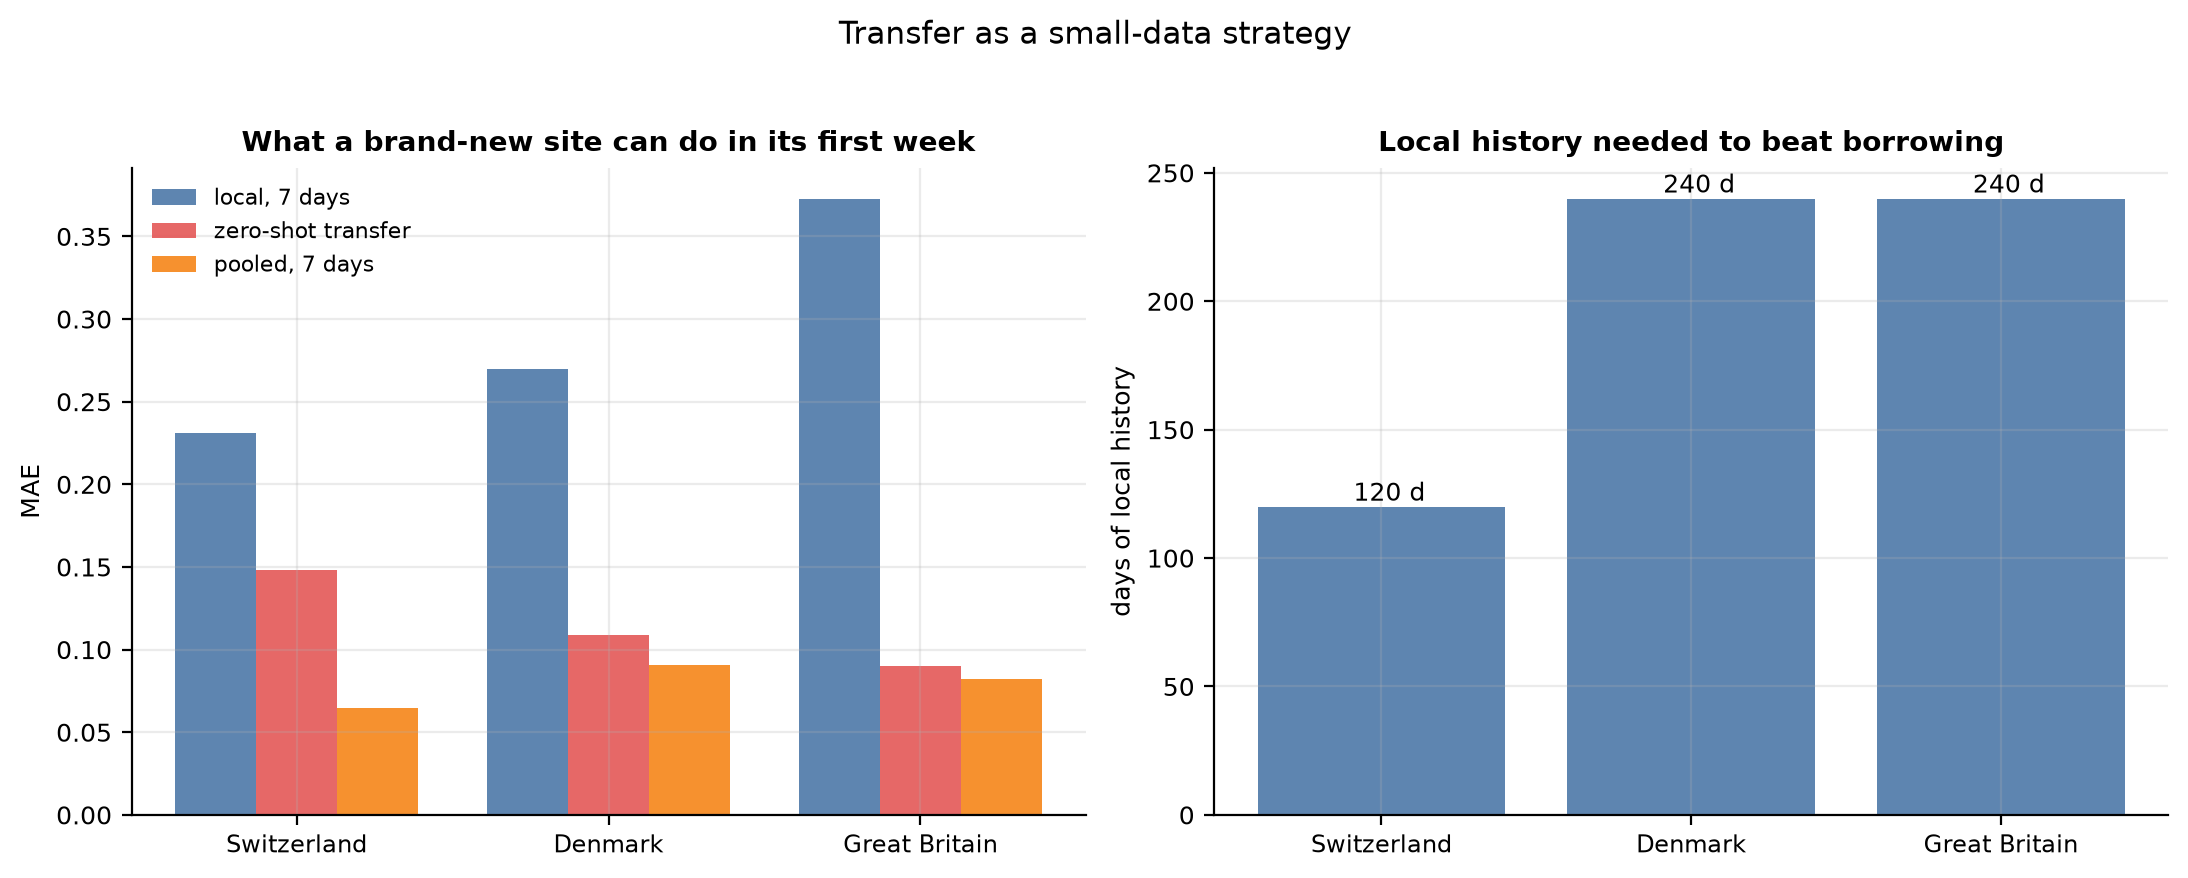
\includegraphics[width=\linewidth]{../figures/15_transfer_summary.png}
\caption{Left, what is achievable in a new site's first week under each strategy. Right, the local history required before training locally overtakes borrowing. The operational reading of the left panel is that the first week is not a period of poor forecasts to be endured, but a period in which a borrowed model performs about as well as it ever will.}
\label{fig:transfer_summary}
\end{figure}

\section{What is not reported, and why}

Three things are deliberately absent. No statistical significance tests are reported across models, because with three folds the fold-to-fold standard errors already show that the leading configurations are not separable and a test would add false precision rather than information. No hyperparameter search is reported, because the study's claims concern the comparison between model classes and between commitment policies rather than the best attainable score, and a search would have consumed the compute budget that the sensitivity grid uses more informatively. No results are reported for the load or wind targets, although the pipeline supports both, because the dispatch problem is posed around PV uncertainty and adding a second uncertain quantity would confound the attribution of regret.


\chapter{Discussion}

\section{Why a linear model won, and what that means}

The leading configuration on both CRPS and MAE is a ridge regression. That is an uncomfortable result to report in a study that also fits gradient-boosted trees and a recurrent network, and it is worth stating plainly rather than burying in a table.

The explanation is that the feature construction has already done the modelling. The physical block supplies the exact deterministic envelope; the gated lags supply the persistence signal; the rolling clear-sky-index statistics supply the atmospheric state. What remains after those three blocks is close to linear in the features provided, and the residual is dominated by tomorrow's cloud cover, which none of the models can see. Additional model capacity has nothing left to spend itself on.

The correct reading is therefore not that boosting is inferior for this problem class, but that on this problem the return to feature engineering exceeded the return to model capacity, and that the fold-to-fold standard errors place the leading configurations in a cluster rather than a ranking. A study with more folds, or with NWP input restoring genuine nonlinear structure, could easily order them differently.

The LSTM's position level with persistence deserves the same care. One to three years of hourly data is a small sample for a sequence model, and two implementation defects had to be corrected before the number could be trusted at all. The honest conclusion is that this dataset is too small for the architecture, not that the architecture is unsuited to the problem.

\section{Calibration is cheap, and validity is not the same as marginal validity}

The strongest practical recommendation in this report is the least novel one: calibrate. Conformal calibration required a ninety-day held-out slice and negligible compute, and it improved the interval score of every quantile-capable model, by 57 percent for the worst-calibrated of them. Anyone shipping predictive intervals from a quantile model without such a step is shipping intervals whose stated level is decorative.

The more interesting result is the second-order one. Split conformal delivered its guarantee exactly as advertised: marginal coverage of 0.904 against a 0.90 target. It nonetheless failed in a way that matters operationally, dropping to 81 percent coverage in its worst month. The guarantee was never violated; it was simply the wrong guarantee for the use case. An operator does not experience the average of the year. An operator experiences January, and then February.

This is where the seasonality that makes the problem hard also makes the standard tool insufficient, and where adaptive conformal inference earns its place. That it recovered conditional coverage while producing \emph{narrower} intervals on average is the part worth emphasising: the improvement did not come from more conservatism, it came from allocating width to the periods that needed it and withdrawing it from the periods that did not.

\section{Forecast score is a proxy for value, not a substitute}

The correlation of 0.884 between CRPS and dispatch regret is high enough to justify using a scoring rule for model selection during development, and low enough that a final model choice should be validated against the decision. It is also, as Section 5.2 notes, inflated by the presence of one very poor model at the end of both axes; over the narrower set of configurations an analyst would actually be choosing between, the relationship is weaker than the headline number suggests. The inversion observed between the raw and conformalised boosted models is instructive: calibration improved the forecast on a proper scoring rule and very slightly worsened the decision, because the decision in question is a commitment quantile whose optimal value is not the one the calibration targeted.

The wider point is that the mapping from distribution to decision passes through the cost structure. Two forecasters with identical CRPS can produce different decisions if their errors are distributed differently across the quantile the decision reads from. Reporting only the scoring rule leaves that entirely invisible.

\section{Over-hedging is a real and expensive mistake}

Both risk-averse policies lost money relative to the naive point commitment, and they did so while succeeding at their stated objective. CVaR and the fixed conservative quantile each halved the energy shortfall. They simply purchased that reduction at a day-ahead price higher than the imbalance penalty they avoided.

This is a failure mode with an obvious path into production. An operator monitoring imbalance volume, which is the natural thing to monitor because it is visible and unpleasant, would see the risk-averse policy performing well. The cost is diffuse, spread across every hour of the day-ahead schedule, and does not announce itself. The lesson is that the objective must be total cost, and that any intermediate metric adopted as a proxy should be checked against it before it becomes a target.

The commitment-quantile sweep gives the constructive version of the same point. The empirically optimal fixed quantile of 0.55 beat all five of the more sophisticated policies. Where a full stochastic program is not available, tuning one number against realised cost captures most of the value.

\section{A hypothesis the data refuted}

The sensitivity study was designed to test a specific prior expectation: that storage \emph{substitutes} for forecast quality. The reasoning was straightforward. A battery buys after the fact the same insurance that a conservative commitment buys in advance, so an operator with a large battery should need the predictive distribution less, and the advantage of the stochastic policy should decline as storage grows.

The data contradict this. At the high-penalty end of the grid the advantage rises monotonically with battery size, from 17.9 percent with no storage to 35.3 percent at eight megawatt-hours. The mechanism is recourse. With no battery there is nothing to re-optimise once PV is realised, so knowing the full distribution mostly shifts the commitment and little else; with a large battery, the second-stage problem has real freedom, and a scenario-based commitment can position the schedule so that the battery is able to exploit it. The point forecast never asks the battery to do this, because it plans for a single trajectory. Storage and probabilistic forecasting are therefore complements rather than substitutes, at least in the regime where imbalance is expensive enough to matter.

Two qualifications are necessary. The surface is not monotonic in the middle of the penalty range, and at ninety delivery days per cell the individual estimates carry meaningful sampling noise. The high-penalty trend is clear and is supported by a mechanism; the mid-range structure should not be over-interpreted.

\section{Attribution answers a different question than necessity}

The divergence between SHAP attribution and ablation is, in retrospect, exactly what one should expect under feature redundancy, but it is not what a reader of the attribution alone would conclude. Solar geometry genuinely explains most of the variance in PV output, and SHAP correctly assigns it most of the credit for the model's predictions. It is nonetheless removable, because the same deterministic shape is recoverable from the calendar and autoregressive blocks. The cloud-state features explain little variance and receive little attribution, but nothing else in the feature set can stand in for them.

The practical consequence concerns what an organisation chooses to collect and maintain. An engineer reading the attribution table alone would prioritise the physical pipeline and deprioritise the rolling statistics, and would be exactly wrong. Attribution describes what a fitted model leaned on; ablation describes what the problem requires. Under redundancy, which is the normal case rather than an exotic one, only the second supports a resourcing decision.

\section{Borrowing beats collecting, for longer than expected}

The transfer result is the most directly actionable finding in the report, and it inverts the intuition that a new site should wait for data.

The reason it works is that almost everything site-specific has been removed before the learner sees anything. Capacity is divided out, and the clear-sky block is recomputed from the target's own latitude and longitude, so a model trained in Germany and applied in Switzerland is not being asked to generalise across latitude at all --- the astronomy has already been adjusted. What is being transferred is the conditional relationship between recent atmospheric state and tomorrow's output, and that relationship is evidently close to invariant across nine degrees of latitude and three climates.

The corollary is a design principle rather than a result: how much a model transfers is largely a property of how its features were constructed. A model built on raw megawatts and absolute solar angles would transfer nowhere, and no amount of transfer-learning machinery would rescue it.

That pooling dominates fine-tuning is also worth noting, because fine-tuning is the more fashionable option. The fine-tune strategy here corrects the source prediction with a locally fitted linear term, and it needs enough local data to fit that correction reliably --- which is precisely what a new site does not have. Pooling asks a weaker question of the local data: not ``what is systematically different here'' but ``which of the source patterns apply''. On a fortnight of data the weaker question is the answerable one.

\section{What building this pipeline taught about building such pipelines}

Six defects reached working code during development, each producing plausible output. Four are worth generalising from.

The leakage defects were caught by an adversarial test rather than by review, and would not have been caught by review: both involved arithmetic that is correct in the common case and wrong at a boundary. The general form of the test, corrupting data that a computation must not depend on and asserting the output does not move, is applicable well beyond time-series feature construction and costs little to write.

The dispatch defect, in which a terminal state-of-charge obligation was enforced when committing but not when settling, was caught by an implausible number rather than by a test. The stochastic policy appeared 192 percent worse than the point policy at the largest battery size. The signal was that the anomaly appeared only in one corner of a parameter sweep, which is characteristic of an asymmetry in the problem formulation rather than of noise. Sweeping parameters is usually framed as a robustness exercise; here it functioned as a debugging tool.

The most instructive defect is the one in which the recurrent model received an all-zero encoder input for 100 percent of test rows. It did not crash, did not warn, and produced smooth and superficially reasonable forecasts. It was detectable only because it scored worse than seasonal persistence. That is the argument for carrying naive baselines all the way through to the final results table rather than dropping them once the learned models start winning: their function is not only to contextualise the score but to act as a floor below which something is definitely broken.

The sixth defect was found by adding a second boosting library. A clear-sky ratio divided by a denominator that passes through arbitrarily small positive values at twilight reached $4\times10^{197}$: finite, so every NaN and infinity check in the pipeline passed it through, and tolerated silently by LightGBM, which had been the only backend. XGBoost refused the matrix outright. The value had been in the feature block from the beginning and had simply never been asked a question it could not answer. The general lesson is that a second implementation is a cheap correctness test as well as a comparison, and that ``finite'' is a weaker guarantee than it looks in a feature pipeline.


\chapter{Limitations and Threats to Validity}

\section{The NWP-free constraint is self-imposed}

Numerical weather prediction would substantially improve day-ahead PV forecasting skill, and its absence caps everything reported in Chapter 5. The claim made here is about what is achievable without it, which is the relevant question for an operator who cannot buy it, and not that the constraint is optimal. A comparison against an NWP-consuming forecaster on the same site and period would sharpen the contribution and is the obvious next step.

\section{National aggregate rather than a single site}

The target is aggregate German PV output, which is far smoother than any individual installation because it averages over roughly half a million systems and the whole country's weather. Absolute error figures are therefore optimistic for a rooftop or a single park, perhaps substantially so. The relative comparisons between models, between calibration methods and between commitment policies are not affected by this, since all are computed on the same series, but the euro figures should be read as illustrating a mechanism rather than as a site-level forecast of profit.

\section{Load and price uncertainty are excluded}

Load is treated as known and follows a fixed synthetic profile, and prices follow a realistic but synthetic time-of-use tariff rather than settled market data. This isolates PV uncertainty, which is the object of study, at the cost of understating total regret. It probably also understates the advantage of the stochastic commitment, since a second uncertain quantity would give the scenario formulation more to work with.

\section{Three folds is a small number}

The backtest has three expanding folds, giving three observations per model for the fold-to-fold standard error. Those standard errors are reported precisely because they are large enough to make the top of the leaderboard a cluster. No claim in this report should be read as establishing an ordering among the leading configurations.

\section{The sensitivity grid is noisy}

Each cell of the penalty-by-storage grid rests on ninety delivery days, which is enough to establish the high-penalty trend and its mechanism but not enough to support the non-monotonic structure visible in the middle of the range. That structure is reported because suppressing it would misrepresent the evidence, but it is not interpreted.

\section{The transfer study rests on three targets and one source}

Three target zones, one source and one base learner is enough to establish that transfer works here and to locate the crossover, but not enough to characterise how either depends on the source-target relationship. The natural next question --- whether a Mediterranean source transfers to a Nordic target as readily as the reverse --- needs a full source-by-target grid rather than a single column of it. The three targets also share the constraint of being northern European; nothing here speaks to transferring across a genuinely different solar regime.

The comparison also normalises every site by the 99.9th percentile of its own generation rather than by capacity, because only Germany's reported capacity is coherent with its own generation series. That scale is well defined and comparable across sites, but it is not a capacity factor, so the transfer MAE figures are not directly comparable with the capacity-factor MAE figures in Section 5.1.

\section{Not every method named in the brief is implemented}

The brief for this topic lists temporal convolutional networks, the Temporal Fusion Transformer (qualified as ``if advanced'') and metaheuristics alongside the methods used here. None of the three is implemented, and the omissions are of two different kinds.

TCN and TFT are genuine gaps. The LSTM result in Section 5.1 suggests why they were not pursued -- a sequence model on one to three years of hourly data lands level with persistence, and a larger architecture on the same data would more likely widen that gap than close it -- but that is an argument for expecting little, not evidence that little is there.

The metaheuristic omission is a deliberate substitution. Metaheuristics are search procedures for problems without exploitable structure, and the dispatch problem here is a linear program: HiGHS returns a certified global optimum in about 0.16 seconds. A metaheuristic could only approximate what is already solved exactly, so applying one would demonstrate the method rather than improve the result.

\section{One run, one seed}

All experiments are seeded and reproducible, but each is run once. Variance across seeds is not estimated. This matters most for the LSTM, whose initialisation and minibatch ordering are stochastic, and least for the linear and tree models, which are close to deterministic given the data.

\section{The drift result rests on a single detected event}

The drift-triggered policy fired once over a two-year test period. That is enough to demonstrate that a properly scaled detector can allocate a retraining budget more efficiently than a calendar, but it is not enough to characterise the detector's precision or recall on this signal. A longer series, or a semi-synthetic series with injected change points of known location, would be required for that.

\section{Detector thresholds were adjusted after seeing the data}

The detector standardisation described in Section 5.3 was introduced after the first run produced zero triggers. This is a legitimate correction of a scale-compatibility defect rather than a tuning of thresholds to improve a result, and the regression test pins the property that motivated it. It is nonetheless a change made with knowledge of the data, and is recorded here as such.


\chapter{Conclusion and Outlook}

\section{What was built}

An end-to-end, reproducible pipeline that takes an openly licensed hourly generation series, constructs a leakage-audited day-ahead design matrix without any weather input, fits six families of forecaster under one interface, calibrates their predictive intervals both classically and adaptively, and then spends those intervals in a two-stage stochastic dispatch problem whose output is denominated in euros. The same backtest output feeds the drift and explainability studies, so all four research questions are answered on one pipeline rather than on four.

\section{What was found}

Raw quantile intervals are not valid, covering as little as 22.5 percent at a nominal 90 percent when built from in-sample residuals, and conformal calibration repairs this cheaply. Marginal validity is not sufficient: split conformal met its guarantee while dropping to 81 percent coverage in its worst month, and adaptive conformal inference recovered conditional coverage while producing narrower intervals.

Forecast score and decision value correlate at $r = 0.884$ across twenty configurations, closely enough to be useful and loosely enough to invert on individual pairs -- and that figure is itself sensitive to which models are in the comparison. The value of committing against a full predictive distribution rather than a point forecast ranged from 3 to 67 percent of regret depending on the imbalance penalty and the storage available, which means no single figure for that value is meaningful without stating both. Risk-averse commitment policies lost money while succeeding at reducing imbalance volume.

For a newly commissioned site, borrowing beats collecting for far longer than expected. A model trained on Germany and applied unchanged to Switzerland, Denmark or Great Britain beat a locally trained model until the local site had accumulated between four and eight months of history. Pooling the source and local data together was better still, and at two of the three sites pooled training on one week of local history beat local-only training on sixteen months.

Two baselines settled questions rather than competing: Prophet, being univariate, finished last by a wide margin at $-$60 percent skill against persistence, and the choice between LightGBM and XGBoost changed nothing measurable.

Drift-triggered retraining achieved the best accuracy of the three policies while spending two refits against a calendar policy's seven, but only after the detectors were made scale-free; in their default configuration they were structurally incapable of firing on a signal of this magnitude.

The feature family carrying two-thirds of SHAP attribution was entirely removable, and the family carrying 8.5 percent was not.

\section{What this says about the field}

Two themes recur. The first is that guarantees should be read carefully: a method can deliver exactly what it promises and still be the wrong tool, as split conformal was here. The second is that intermediate metrics drift away from objectives, and that the drift is invisible unless the objective is measured directly. Both the CVaR result and the SHAP result are instances of a metric behaving well while the thing it stood for behaved badly.

\section{Future work}

The transfer result suggests its own extension: a full source-by-target grid across the twenty-odd European zones in the same data package would turn a single demonstration into a map of which sites are worth borrowing from, and the divergence bound of Ben-David et al. gives a principled quantity to correlate that map against.

Four further directions follow directly. Adding NWP input would establish how much of the ceiling observed here is attributable to the missing weather model. Extending the uncertainty treatment to load and price would give the stochastic formulation a fairer test. Replacing the synthetic tariff with settled market data would make the euro figures site-specific rather than illustrative. Finally, evaluating on individual sites rather than a national aggregate would establish whether the conclusions about calibration and decision value survive the much noisier signal that a single installation produces, which is the setting in which they would actually be applied.


\chapter{References}


Every entry below was verified against a live bibliographic source (Crossref, OpenAlex or arXiv) rather than written from memory. Formatting follows APA 7.

Angelopoulos, A. N., \& Bates, S. (2023). Conformal prediction: A gentle introduction. \emph{Foundations and Trends in Machine Learning, 16}(4), 494-591. \href{https://doi.org/10.1561/2200000101}{https://doi.org/10.1561/2200000101}

Antonanzas, J., Osorio, N., Escobar, R., Urraca, R., Martinez-de-Pison, F. J., \& Antonanzas-Torres, F. (2016). Review of photovoltaic power forecasting. \emph{Solar Energy, 136}, 78-111. \href{https://doi.org/10.1016/j.solener.2016.06.069}{https://doi.org/10.1016/j.solener.2016.06.069}

Bifet, A., \& Gavald\`a, R. (2007). Learning from time-changing data with adaptive windowing. \emph{Proceedings of the 2007 SIAM International Conference on Data Mining}, 443-448. \href{https://doi.org/10.1137/1.9781611972771.42}{https://doi.org/10.1137/1.9781611972771.42}

Ben-David, S., Blitzer, J., Crammer, K., Kulesza, A., Pereira, F., \& Vaughan, J. W. (2010). A theory of learning from different domains. \emph{Machine Learning, 79}(1-2), 151-175. \href{https://doi.org/10.1007/s10994-009-5152-4}{https://doi.org/10.1007/s10994-009-5152-4}

Bremnes, J. B. (2004). Probabilistic wind power forecasts using local quantile regression. \emph{Wind Energy, 7}(1), 47-54. \href{https://doi.org/10.1002/we.107}{https://doi.org/10.1002/we.107}

Chen, T., \& Guestrin, C. (2016). XGBoost: A scalable tree boosting system. \emph{Proceedings of the 22nd ACM SIGKDD International Conference on Knowledge Discovery and Data Mining}, 785-794. \href{https://doi.org/10.1145/2939672.2939785}{https://doi.org/10.1145/2939672.2939785}

Chernozhukov, V., Fern\'andez-Val, I., \& Galichon, A. (2010). Quantile and probability curves without crossing. \emph{Econometrica, 78}(3), 1093-1125. \href{https://doi.org/10.3982/ECTA7880}{https://doi.org/10.3982/ECTA7880}

Gama, J., \v{Z}liobait\.e, I., Bifet, A., Pechenizkiy, M., \& Bouchachia, A. (2014). A survey on concept drift adaptation. \emph{ACM Computing Surveys, 46}(4), 1-37. \href{https://doi.org/10.1145/2523813}{https://doi.org/10.1145/2523813}

Gibbs, I., \& Cand\`es, E. J. (2021). Adaptive conformal inference under distribution shift. \emph{Advances in Neural Information Processing Systems, 34}. arXiv:2106.00170. \href{https://arxiv.org/abs/2106.00170}{https://arxiv.org/abs/2106.00170}

Gneiting, T., \& Katzfuss, M. (2014). Probabilistic forecasting. \emph{Annual Review of Statistics and Its Application, 1}, 125-151. \href{https://doi.org/10.1146/annurev-statistics-062713-085831}{https://doi.org/10.1146/annurev-statistics-062713-085831}

Gneiting, T., \& Raftery, A. E. (2007). Strictly proper scoring rules, prediction, and estimation. \emph{Journal of the American Statistical Association, 102}(477), 359-378. \href{https://doi.org/10.1198/016214506000001437}{https://doi.org/10.1198/016214506000001437}

Haurwitz, B. (1945). Insolation in relation to cloudiness and cloud density. \emph{Journal of Meteorology, 2}(3), 154-166. \href{https://doi.org/10.1175/1520-0469(1945)002<0154:IIRTCA>2.0.CO;2}{https://doi.org/10.1175/1520-0469(1945)002$<$0154:IIRTCA$>$2.0.CO;2}

Hong, T., Pinson, P., Fan, S., Zareipour, H., Troccoli, A., \& Hyndman, R. J. (2016). Probabilistic energy forecasting: Global Energy Forecasting Competition 2014 and beyond. \emph{International Journal of Forecasting, 32}(3), 896-913. \href{https://doi.org/10.1016/j.ijforecast.2016.02.001}{https://doi.org/10.1016/j.ijforecast.2016.02.001}

Huangfu, Q., \& Hall, J. A. J. (2018). Parallelizing the dual revised simplex method. \emph{Mathematical Programming Computation, 10}(1), 119-142. \href{https://doi.org/10.1007/s12532-017-0130-5}{https://doi.org/10.1007/s12532-017-0130-5}

Ineichen, P., \& Perez, R. (2002). A new airmass independent formulation for the Linke turbidity coefficient. \emph{Solar Energy, 73}(3), 151-157. \href{https://doi.org/10.1016/S0038-092X(02)00045-2}{https://doi.org/10.1016/S0038-092X(02)00045-2}

Kasten, F., \& Young, A. T. (1989). Revised optical air mass tables and approximation formula. \emph{Applied Optics, 28}(22), 4735-4738. \href{https://doi.org/10.1364/AO.28.004735}{https://doi.org/10.1364/AO.28.004735}

Ke, G., Meng, Q., Finley, T., Wang, T., Chen, W., Ma, W., Ye, Q., \& Liu, T.-Y. (2017). LightGBM: A highly efficient gradient boosting decision tree. \emph{Advances in Neural Information Processing Systems, 30}, 3146-3154.

Koenker, R., \& Bassett, G. (1978). Regression quantiles. \emph{Econometrica, 46}(1), 33-50. \href{https://doi.org/10.2307/1913643}{https://doi.org/10.2307/1913643}

Lim, B., Ar\i k, S. \"O., Loeff, N., \& Pfister, T. (2021). Temporal Fusion Transformers for interpretable multi-horizon time series forecasting. \emph{International Journal of Forecasting, 37}(4), 1748-1764. \href{https://doi.org/10.1016/j.ijforecast.2021.03.012}{https://doi.org/10.1016/j.ijforecast.2021.03.012}

Lundberg, S. M., \& Lee, S.-I. (2017). A unified approach to interpreting model predictions. \emph{Advances in Neural Information Processing Systems, 30}. arXiv:1705.07874. \href{https://arxiv.org/abs/1705.07874}{https://arxiv.org/abs/1705.07874}

Luo, X., Zhang, D., \& Zhu, X. (2022). Combining transfer learning and constrained long short-term memory for power generation forecasting of newly-constructed photovoltaic plants. \emph{Renewable Energy, 185}, 1062-1077. \href{https://doi.org/10.1016/j.renene.2021.12.104}{https://doi.org/10.1016/j.renene.2021.12.104}

Morales, J. M., Conejo, A. J., Madsen, H., Pinson, P., \& Zugno, M. (2014). \emph{Integrating renewables in electricity markets: Operational problems}. Springer. \href{https://doi.org/10.1007/978-1-4614-9411-9}{https://doi.org/10.1007/978-1-4614-9411-9}

Open Power System Data. (2020). \emph{Time series} (Version 2020-10-06) [Data set]. \href{https://doi.org/10.25832/time_series/2020-10-06}{https://doi.org/10.25832/time\_series/2020-10-06}

Pan, S. J., \& Yang, Q. (2010). A survey on transfer learning. \emph{IEEE Transactions on Knowledge and Data Engineering, 22}(10), 1345-1359. \href{https://doi.org/10.1109/TKDE.2009.191}{https://doi.org/10.1109/TKDE.2009.191}

Pinson, P. (2012). Very-short-term probabilistic forecasting of wind power with generalized logit-normal distributions. \emph{Journal of the Royal Statistical Society: Series C, 61}(4), 555-576. \href{https://doi.org/10.1111/j.1467-9876.2011.01026.x}{https://doi.org/10.1111/j.1467-9876.2011.01026.x}

Pinson, P., Chevallier, C., \& Kariniotakis, G. N. (2007). Trading wind generation from short-term probabilistic forecasts of wind power. \emph{IEEE Transactions on Power Systems, 22}(3), 1148-1156. \href{https://doi.org/10.1109/TPWRS.2007.901117}{https://doi.org/10.1109/TPWRS.2007.901117}

Reda, I., \& Andreas, A. (2004). Solar position algorithm for solar radiation applications. \emph{Solar Energy, 76}(5), 577-589. \href{https://doi.org/10.1016/j.solener.2003.12.003}{https://doi.org/10.1016/j.solener.2003.12.003}

Rockafellar, R. T., \& Uryasev, S. (2000). Optimization of conditional value-at-risk. \emph{The Journal of Risk, 2}(3), 21-41. \href{https://doi.org/10.21314/JOR.2000.038}{https://doi.org/10.21314/JOR.2000.038}

Romano, Y., Patterson, E., \& Cand\`es, E. J. (2019). Conformalized quantile regression. \emph{Advances in Neural Information Processing Systems, 32}. arXiv:1905.03222. \href{https://arxiv.org/abs/1905.03222}{https://arxiv.org/abs/1905.03222}

Taylor, S. J., \& Letham, B. (2018). Forecasting at scale. \emph{The American Statistician, 72}(1), 37-45. \href{https://doi.org/10.1080/00031305.2017.1380080}{https://doi.org/10.1080/00031305.2017.1380080}

van der Meer, D. W., Wid\'en, J., \& Munkhammar, J. (2018). Review on probabilistic forecasting of photovoltaic power production and electricity consumption. \emph{Renewable and Sustainable Energy Reviews, 81}, 1484-1512. \href{https://doi.org/10.1016/j.rser.2017.05.212}{https://doi.org/10.1016/j.rser.2017.05.212}

Vovk, V., Gammerman, A., \& Shafer, G. (2022). \emph{Algorithmic learning in a random world} (2nd ed.). Springer. \href{https://doi.org/10.1007/978-3-031-06649-8}{https://doi.org/10.1007/978-3-031-06649-8}

Wang, H., Yi, H., Peng, J., Wang, G., Liu, Y., Jiang, H., \& Liu, W. (2017). Deterministic and probabilistic forecasting of photovoltaic power based on deep convolutional neural network. \emph{Energy Conversion and Management, 153}, 409-422. \href{https://doi.org/10.1016/j.enconman.2017.10.008}{https://doi.org/10.1016/j.enconman.2017.10.008}

Winkler, R. L. (1972). A decision-theoretic approach to interval estimation. \emph{Journal of the American Statistical Association, 67}(337), 187-191. \href{https://doi.org/10.1080/01621459.1972.10481224}{https://doi.org/10.1080/01621459.1972.10481224}

\end{document}
